  %%%%%%%%%%%%%%%%%%%%%%%%%%%%%%%%%%%%%%%%%%%%%%%%%%%%%%%%%%%%%%%%%%%%%%%%%
%%%%%%%%%%%%%%%%%%%%%%%%%%%%%%%%%%%%%%%%%%%%%%%%%%%%%%%%%%%%%%%%%%%%%%%%%
%%%                                                                   %%%
%%%  PLANTILLA DE TRABAJOS DE GRADO UNIVERSIDAD CATÓLICA BOLIVIANA    %%% 
%%%                                                                   %%%
%%%       AUTOR PRINCIPAL TEMPLATE:   RODOLFO JESÚS PRIETO MALDONADO  %%%
%%%       E-MAIL                  :   rodolfo.jp.13@gmail.com         %%%
%%%       AUTOR GUÍA/APOYO        :   EDWIN CALLA DURANDAL            %%%
%%%       E-MAIL                  :   ecalla.d@ucb.edu.bo             %%%
%%%                                   edwin.calla@gmail.com           %%%
%%%       GESTIÓN ELABORACIÓN     :   2 - 2018                        %%%
%%%       COMPILADOR              :   XeLateX                         %%%
%%%     ÚLTIMA ACTUALIZACIÓN      :   06 de Junio de 2020             %%%
%%%                                    Horas 21:00                    %%%
%%%                                                                   %%%
%%%%%%%%%%%%%%%%%%%%%%%%%%%%%%%%%%%%%%%%%%%%%%%%%%%%%%%%%%%%%%%%%%%%%%%%%
%%%%%%%%%%%%%%%%%%%%%%%%%%%%%%%%%%%%%%%%%%%%%%%%%%%%%%%%%%%%%%%%%%%%%%%%%
%
% Junto a las modalidades de titulación y el objetivo que persigue la carrera de Ing. Mecatrónica de formar profesionales íntegros y de alto nivel, se dispone al estudiante el Template de Latex para la elaboración del documento de titulación de la carrera, como también para presentar cualquier tipo de trabajo dentro de la misma.
% 
% IMPORTANTE
% El compilador (Compiler) a ser utilizado debe ser XeLateX
%
% IMPORTANTE
% Los espacios a ser modificados serán identificados de la siguiente forma:

%------------------------
%
%       DEDICATORIA
%
%------------------------

% Los demás espacios y códigos son parte del formato, si se desea modificar los mismos, es bajo la responsabilidad del editor, siendo que podrá alterar el formato de la institución. 
% Caso usted encuentre algún problema de formato u otro tipo, usted encontrará un formulario para reportar cualquier bug (error) en la página web donde se descargo el presente Template. 

% Para comenzar a editar y trabajar, por favor dirigirse a la línea de código del presente archivo número 494 y llenar los espacios necesarios, posterior a esto, dirigirse a dedicatoria, resumen, introducción, marco teórico, marco metodológico, conclusiones, anexos y apéndices. Usted podrá modificar los mismos según sus necesidades. 

%%%%%% NO MODIFICAR %%%%%%% NO MODIFICAR %%%%%%%%%% NO MODIFICAR %%%%%%%%% NO MODIFICAR %%%%%%%%
%%%%%%%%%%%%%%% NO TOCAR %%%%%%%%%%%%% NO TOCAR %%%%%%%%%%%%% NO TOCAR %%%%%%%%%% NO TOCAR %%%%%
%%%%%% NO MODIFICAR %%%%%%%% NO MODIFICAR %%%%%%%%%% NO MODIFICAR %%%%%%% NO MODIFICAR %%%%%%%%%
%%%%%%%%%%% NO TOCA R%%%%%%%%%%%%% NO TOCAR %%%%%%%%%%%%% NO TOCAR %%%%%%%%%%%%%% NO TOCAR %%%%%

% Inicio código formato
%   Condiciones generales   |   tamaño de hoja, tamaño de letra en general
\documentclass[letterpaper,12pt]{article}   % carta, letra 12

%---------- PAQUETES --------------

%  Márgenes
\usepackage[left=3.5cm,right=3cm,top=3cm,bottom=3cm]{geometry}

%% Básicos
\usepackage[spanish]{babel}         % Idioma (silabación y gestión de palabras)
\usepackage{csquotes}               % Reglas del lenguaje

\usepackage{fontspec}               % Fuente Times New Roman
\setmainfont{Arial}
\usepackage{silence}                % Remueve Warnings
\WarningsOff[transparent]

\usepackage{enumitem}               % Habilita enumeración
\usepackage{fancyhdr}               % Cabeceras y pies de página 
\usepackage[table,xcdraw]{xcolor}   % Habilita cambios de color (texto, hoja, etc)
\usepackage{titling}                % Títulos y nombres en el documento
\usepackage{titlesec}               % Edición de formato de secciones
\usepackage{tocloft}                % Índice
\usepackage{setspace}               % Interlineado
\usepackage{lscape}
\usepackage{tikz}
\usetikzlibrary{calc}
\usepackage[linktocpage=true,hidelinks]{hyperref}           % Habilita hipervínculos 

\usepackage{multicol}                                       % MULTIPLE COLUMNAS
\usepackage{multirow}                                       % MULTIPLES FILAS
\usepackage[absolute]{textpos}
\usepackage[acronym,xindy]{glossaries}

\usepackage{array}
\usepackage{makecell}                                       % Eol on tables

\usepackage{svg}
%\usepackage[outline]{contour}

\usepackage{xifthen}                                        % Provides \isempty test
\usepackage{minted}

\usepackage{listings}
\usepackage{xcolor}

\usepackage{listings}
\usepackage{xcolor}

\lstdefinestyle{mypy}{
  language=Python,
  basicstyle=\ttfamily\small,
  numbers=left, numberstyle=\tiny, numbersep=6pt,
  showstringspaces=false,
  breaklines=true,
  frame=single,
  captionpos=t,
  xleftmargin=2em,
  keywordstyle=\color{blue}\bfseries,
  stringstyle=\color{teal!60!black},
  commentstyle=\color{gray!70}\itshape
}

% Definición manual de JavaScript
\lstdefinelanguage{JavaScript}{
  morekeywords={typeof,new,true,false,catch,function,return,null,
    switch,var,if,in,while,do,else,case,break,import,from,export,default},
  keywordstyle=\color{blue}\bfseries,
  ndkeywords={class,export,boolean,throw,implements,import,this},
  ndkeywordstyle=\color{magenta}\bfseries,
  identifierstyle=\color{black},
  sensitive=false,
  comment=[l]{//},
  morecomment=[s]{/*}{*/},
  commentstyle=\color{green!50!black}\ttfamily,
  stringstyle=\color{red!70!black}\ttfamily,
  morestring=[b]',
  morestring=[b]"
}

\lstdefinestyle{javascript}{
  language=JavaScript,
  basicstyle=\ttfamily\small,
  numbers=left,
  numberstyle=\tiny,
  frame=single,
  breaklines=true,
  showstringspaces=false
}






%% Matemáticos
\usepackage{amsmath, amsthm, amssymb, amsfonts, upgreek}
\spanishdecimal{.}

%% Pseudo algoritmos
\usepackage[]{algorithmic,algorithm}
\renewcommand{\algorithmicrequire}{\textbf{Inicio}}
\renewcommand{\algorithmicensure}{\textbf{Fin}}
\usepackage[algo2e,boxed,linesnumbered,ruled,vlined]{algorithm2e}
\floatname{algorithm}{Algoritmo}

%% Código Matlab
\usepackage{listings}
\lstset{language=Matlab, breaklines=true, basicstyle=\footnotesize}
\lstset{numbers=left, numberstyle=\tiny, stepnumber=1, numbersep=-2pt}

\lstset{literate=
  {á}{{\'a}}1 {é}{{\'e}}1 {í}{{\'i}}1 {ó}{{\'o}}1 {ú}{{\'u}}1
  {Á}{{\'A}}1 {É}{{\'E}}1 {Í}{{\'I}}1 {Ó}{{\'O}}1 {Ú}{{\'U}}1
  {à}{{\`a}}1 {è}{{\`e}}1 {ì}{{\`i}}1 {ò}{{\`o}}1 {ù}{{\`u}}1
  {À}{{\`A}}1 {È}{{\'E}}1 {Ì}{{\`I}}1 {Ò}{{\`O}}1 {Ù}{{\`U}}1
  {ä}{{\"a}}1 {ë}{{\"e}}1 {ï}{{\"i}}1 {ö}{{\"o}}1 {ü}{{\"u}}1
  {Ä}{{\"A}}1 {Ë}{{\"E}}1 {Ï}{{\"I}}1 {Ö}{{\"O}}1 {Ü}{{\"U}}1
  {â}{{\^a}}1 {ê}{{\^e}}1 {î}{{\^i}}1 {ô}{{\^o}}1 {û}{{\^u}}1
  {Â}{{\^A}}1 {Ê}{{\^E}}1 {Î}{{\^I}}1 {Ô}{{\^O}}1 {Û}{{\^U}}1
  {Ã}{{\~A}}1 {ã}{{\~a}}1 {Õ}{{\~O}}1 {õ}{{\~o}}1
  {œ}{{\oe}}1 {Œ}{{\OE}}1 {æ}{{\ae}}1 {Æ}{{\AE}}1 {ß}{{\ss}}1
  {ű}{{\H{u}}}1 {Ű}{{\H{U}}}1 {ő}{{\H{o}}}1 {Ő}{{\H{O}}}1
  {ç}{{\c c}}1 {Ç}{{\c C}}1 {ø}{{\o}}1 {å}{{\r a}}1 {Å}{{\r A}}1
  {€}{{\euro}}1 {£}{{\pounds}}1 {«}{{\guillemotleft}}1
  {»}{{\guillemotright}}1 {ñ}{{\~n}}1 {Ñ}{{\~N}}1 {¿}{{?`}}1
}

%% Imágenes
\usepackage{graphicx}           % Inclusión de imágenes
\usepackage{wrapfig}            % Optimiza texto alrededor de las imágenes
\usepackage{float}              % Ubicación inteligente de imágenes 
\usepackage[justification=raggedright,singlelinecheck=false]{caption}           % Habilita edición de títulos de figuras
\usepackage{subfig}             % Habilita edición de sub-figuras

\usepackage{pdfpages}           % Introduce pdf (anexos)
\usepackage{longtable}


%% Extras
\usepackage{verbatim}           % Habilita big-comment y ambientes especiales
\usepackage{lipsum} 
\usepackage{array} 
\usepackage{multirow}
\usepackage{afterpage}          % obliga a una tabla a estar en su lugar
                                %   \afterpage{\clearpage}  usa esto antes de la tabla

% Gestión de bibliografía
\usepackage[backend=biber, style=apa]{biblatex}
\DeclareLanguageMapping{spanish}{spanish-apa}
\addbibresource{bibliografia.bib}

%%%%%% NO MODIFICAR %%%%%%% NO MODIFICAR %%%%%%%%%% NO MODIFICAR %%%%%%%%% NO MODIFICAR %%%%%%%%
%%%%%%%%%%%%%%% NO TOCAR %%%%%%%%%%%%% NO TOCAR %%%%%%%%%%%%% NO TOCAR %%%%%%%%%% NO TOCAR %%%%%
%%%%%% NO MODIFICAR %%%%%%%% NO MODIFICAR %%%%%%%%%% NO MODIFICAR %%%%%%% NO MODIFICAR %%%%%%%%%
%%%%%%%%%%% NO TOCA R%%%%%%%%%%%%% NO TOCAR %%%%%%%%%%%%% NO TOCAR %%%%%%%%%%%%%% NO TOCAR %%%%%

%------- FORMATO ------------------

%grosor fijo de las columnas en las tablas
\newcolumntype{L}[1]{>{\raggedright\let\newline\\\arraybackslash\hspace{0pt}}m{#1}}
\newcolumntype{C}[1]{>{\centering\let\newline\\\arraybackslash\hspace{0pt}}m{#1}}
\newcolumntype{R}[1]{>{\raggedleft\let\newline\\\arraybackslash\hspace{0pt}}m{#1}}
\newcolumntype{J}[1]{>{\let\newline\\\arraybackslash\hspace{0pt}}m{#1}}

% eol onsie tables
\renewcommand\theadalign{bc}
\renewcommand\theadfont{\bfseries}
\renewcommand\theadgape{\Gape[4pt]}
\renewcommand\cellgape{\Gape[4pt]}

%%%%%% NO MODIFICAR %%%%%%% NO MODIFICAR %%%%%%%%%% NO MODIFICAR %%%%%%%%% NO MODIFICAR %%%%%%%%
%%%%%%%%%%%%%%% NO TOCAR %%%%%%%%%%%%% NO TOCAR %%%%%%%%%%%%% NO TOCAR %%%%%%%%%% NO TOCAR %%%%%
%%%%%% NO MODIFICAR %%%%%%%% NO MODIFICAR %%%%%%%%%% NO MODIFICAR %%%%%%% NO MODIFICAR %%%%%%%%%
%%%%%%%%%%% NO TOCA R%%%%%%%%%%%%% NO TOCAR %%%%%%%%%%%%% NO TOCAR %%%%%%%%%%%%%% NO TOCAR %%%%%

% --------- Formato de Índices ---------
\renewcommand{\cftdotsep}{0.5}

% Sangrías
\renewcommand{\cftsubsecindent}{0em}
\renewcommand{\cftsubsubsecindent}{0em}
\renewcommand{\cftparaindent}{0em}

% Puntos de conexión (líderes)
\renewcommand{\cftsecleader}{\cftdotfill{\cftdotsep}}
\renewcommand{\cftfigleader}{\cftdotfill{\cftdotsep}}
\renewcommand{\cfttableader}{\cftdotfill{\cftdotsep}}

% Puntos tras número
\renewcommand{\cftsecaftersnum}{.}
\renewcommand{\cftsubsecaftersnum}{.}
\renewcommand{\cftsubsubsecaftersnum}{.}
\renewcommand{\cftparaaftersnum}{.}
\renewcommand{\cftsubparaaftersnum}{.}

% Título centrado y en mayúsculas
\renewcommand{\cfttoctitlefont}{\hspace*{\fill}\normalsize\bfseries\MakeUppercase}
\renewcommand{\cftaftertoctitle}{\hspace*{\fill}}
\renewcommand{\cftlottitlefont}{\hspace*{\fill}\normalsize\bfseries\MakeUppercase}
\renewcommand{\cftafterlottitle}{\hspace*{\fill}}
\renewcommand{\cftloftitlefont}{\hspace*{\fill}\normalsize\bfseries\MakeUppercase}
\renewcommand{\cftafterloftitle}{\hspace*{\fill}}

% Espaciado antes de cada nivel
\setlength{\cftbeforesecskip}{4pt}
\setlength{\cftbeforesubsecskip}{2pt}
\setlength{\cftbeforesubsubsecskip}{1pt}
\setlength{\cftbeforeparaskip}{1pt}
\setlength{\cftbeforesubparaskip}{1pt}
\setlength{\cftbeforefigskip}{2pt}
\setlength{\cftbeforetabskip}{2pt}

% Formato de fuente por nivel
\renewcommand{\cftsecfont}{\normalfont}              % Secciones en negrita
\renewcommand{\cftsubsecfont}{\normalfont}           % Subsecciones normal
\renewcommand{\cftsubsubsecfont}{\normalfont}        % Subsubsecciones normal
\renewcommand{\cftparafont}{\normalfont\itshape}     % Párrafos en cursiva
\renewcommand{\cftsubparafont}{\normalfont\itshape}  % Subpárrafos en cursiva

% Números de página en texto normal
\renewcommand{\cftsecpagefont}{\normalfont}

% Personalización de figuras y tablas
\cftsetindents{figure}{0em}{5em}
\renewcommand{\cftfigpresnum}{\bfseries Figura }

\cftsetindents{table}{0em}{4.6em}
\renewcommand{\cfttabpresnum}{\bfseries Tabla }

%-----------Referenciación-------------------------
\hypersetup{
    colorlinks=false, %set true if you want colored links
    linktoc=all,      %set to all if you want both sections and subsections linked
    linkcolor=black,  %choose some color if you want links to stand out
}

%%%%%% NO MODIFICAR %%%%%%% NO MODIFICAR %%%%%%%%%% NO MODIFICAR %%%%%%%%% NO MODIFICAR %%%%%%%%
%%%%%%%%%%%%%%% NO TOCAR %%%%%%%%%%%%% NO TOCAR %%%%%%%%%%%%% NO TOCAR %%%%%%%%%% NO TOCAR %%%%%
%%%%%% NO MODIFICAR %%%%%%%% NO MODIFICAR %%%%%%%%%% NO MODIFICAR %%%%%%% NO MODIFICAR %%%%%%%%%
%%%%%%%%%%% NO TOCA R%%%%%%%%%%%%% NO TOCAR %%%%%%%%%%%%% NO TOCAR %%%%%%%%%%%%%% NO TOCAR %%%%%

%-------------Comandos de citación-----------------------
\newbibmacro*{cite:labelyear+extrayear}{%
\iffieldundef{labelyear}
{}
{\printtext[bibhyperref]{%
\printfield{labelyear}%
\printfield{extrayear}}}}

\newbibmacro*{cite:authoryear}{%
\printnames[][-\value{listtotal}]{labelname}
\setunit*{\printdelim{nameyeardelim}}%
\printtext[bibhyperlink]{%
\usebibmacro{cite:labelyear}}}

\newbibmacro*{cite:authoryear2}{%
Cf. \printnames[][-\value{listtotal}]{labelname}
\setunit*{\printdelim{nameyeardelim}}%
\printtext[bibhyperlink]{%
\usebibmacro{cite:labelyear}}}

\newbibmacro*{cite:authoryear3}{%
\printnames[][-\value{listtotal}]{labelname}
\printtext[bibhyperlink]{%
(\usebibmacro{cite:labelyear}}}

\newbibmacro*{cite:authoryear4}{%
\printnames[][-\value{listtotal}]{labelname}
\printtext[bibhyperlink]{%
\usebibmacro{cite:labelyear}}}

\DeclareCiteCommand{\cite}[]
  {\usebibmacro{prenote}}
  {\usebibmacro{citeindex}%
   \printtext[bibhyperref]{\usebibmacro{cite:authoryear3}}}
  {\multicitedelim}
  {\usebibmacro{postnote})}

\DeclareCiteCommand*{\cite}[]
  {\usebibmacro{prenote}}
  {\usebibmacro{citeindex}%
   \printtext[bibhyperref]{\usebibmacro{cite:authoryear3}}}
  {\multicitedelim}
  {\usebibmacro{postnote}}
  
  \DeclareCiteCommand{\citel}[]
  {\usebibmacro{prenote}}
  {\usebibmacro{citeindex}%
   \printtext[bibhyperref]{\usebibmacro{cite:authoryear4}}}
  {\multicitedelim}
  {\usebibmacro{postnote}}

\DeclareCiteCommand*{\citel}[]
  {\usebibmacro{prenote}}
  {\usebibmacro{citeindex}%
   \printtext[bibhyperref]{\usebibmacro{cite:authoryear4}}}
  {\multicitedelim}
  {\usebibmacro{postnote}}

\DeclareCiteCommand{\citep}[\mkbibparens]
  {\usebibmacro{prenote}}
  {\usebibmacro{citeindex}%
   \printtext[bibhyperref]{\usebibmacro{cite:authoryear}}}
  {\multicitedelim}
  {\usebibmacro{postnote}}

\DeclareCiteCommand*{\citep}[\mkbibparens]
  {\usebibmacro{prenote}}
  {\usebibmacro{citeindex}%
   \printtext[bibhyperref]{\usebibmacro{cite:authoryear}}}
  {\multicitedelim}
  {\usebibmacro{postnote}}
  
  \DeclareCiteCommand{\citecf}[\mkbibparens]
  {\usebibmacro{prenote}}
  {\usebibmacro{citeindex}%
   \printtext[bibhyperref]{\usebibmacro{cite:authoryear2}}}
  {\multicitedelim}
  {\usebibmacro{postnote}}

\DeclareCiteCommand*{\citecf}[\mkbibparens]
  {\usebibmacro{prenote}}
  {\usebibmacro{citeindex}%
   \printtext[bibhyperref]{\usebibmacro{cite:authoryear2}}}
  {\multicitedelim}
  {\usebibmacro{postnote}}
  
    \renewcommand*{\postnotedelim}{\addcolon\addspace}
    \DeclareFieldFormat{postnote}{#1}
    \DeclareFieldFormat{multipostnote}{#1}

%%%%%% NO MODIFICAR %%%%%%% NO MODIFICAR %%%%%%%%%% NO MODIFICAR %%%%%%%%% NO MODIFICAR %%%%%%%%
%%%%%%%%%%%%%%% NO TOCAR %%%%%%%%%%%%% NO TOCAR %%%%%%%%%%%%% NO TOCAR %%%%%%%%%% NO TOCAR %%%%%
%%%%%% NO MODIFICAR %%%%%%%% NO MODIFICAR %%%%%%%%%% NO MODIFICAR %%%%%%% NO MODIFICAR %%%%%%%%%
%%%%%%%%%%% NO TOCA R%%%%%%%%%%%%% NO TOCAR %%%%%%%%%%%%% NO TOCAR %%%%%%%%%%%%%% NO TOCAR %%%%%

%---------------Formato de títulos------------------------------------
\titleformat{\section}
{\normalsize\bfseries}{\thesection.}{1em}{}

\titleformat{\subsection}
{\normalsize\bfseries}{\thesubsection.}{1em}{}

\titleformat{\subsubsection}
{\normalsize\bfseries\itshape}{\thesubsubsection.}{1em}{}

\setcounter{tocdepth}{4}%
\setcounter{secnumdepth}{5}%

\titleformat{\paragraph}
{\normalsize\itshape}{\theparagraph.}{1em}{}

\titleformat{\subparagraph}
{\normalsize\itshape}{\thesubparagraph.}{1em}{}

\titlespacing*{\section}
{0pt}{0pt}{0pt}
\titlespacing*{\subsection}
{0pt}{0pt}{0pt}
\titlespacing*{\subsubsection}
{0pt}{0pt}{0pt}
\titlespacing*{\paragraph}
{0pt}{0pt}{0pt}
\titlespacing*{\subparagraph}
{0pt}{0pt}{0pt}

%%%%%% NO MODIFICAR %%%%%%% NO MODIFICAR %%%%%%%%%% NO MODIFICAR %%%%%%%%% NO MODIFICAR %%%%%%%%
%%%%%%%%%%%%%%% NO TOCAR %%%%%%%%%%%%% NO TOCAR %%%%%%%%%%%%% NO TOCAR %%%%%%%%%% NO TOCAR %%%%%
%%%%%% NO MODIFICAR %%%%%%%% NO MODIFICAR %%%%%%%%%% NO MODIFICAR %%%%%%% NO MODIFICAR %%%%%%%%%
%%%%%%%%%%% NO TOCA R%%%%%%%%%%%%% NO TOCAR %%%%%%%%%%%%% NO TOCAR %%%%%%%%%%%%%% NO TOCAR %%%%%

%--------Formato de Figuras----------
\graphicspath{ {Figuras/} }     % Buscar figuras en la carpeta Figuras

                    
\captionsetup[figure]           % Formato de figura
{labelfont={bf},labelformat={default},labelsep=newline,name={Figura}}

    \newcommand{\figura}[4][width=\textwidth]       % comando figura
    {
        \begin{figure}[!htb]                        % si la fig se mueve usar [h]
            \centering                              % centrado
            \caption{#3}                   % titulo de la fig
            \includegraphics[#1]{#2}                % figura
            \par
            \centering{\textbf{Fuente:} #4}                  % fuente
            \label{fig:#2}                          % referencia
        \end{figure}
    }
    
\begin{comment}

\begin{figure}[hpt]
    \centering
    
    % Título de figura
    \caption{Título Figura}
        % imagen 1
        %           Título                              Tamaño              nombre img
        \subfloat[titulo de img 1]{\includegraphics[width=0.4\columnwidth]{nombre_img_1}}
        
        % separaciones | agregar una de las opciones entre cada par de imágenes
            \qquad      % figuras en la misma linea
            \par        % siguiente línea
            
        % imagen 2
        %           Título                              Tamaño              nombre img
        \subfloat[título de img 2]{\includegraphics[width=0.4\columnwidth]{nombre_img_2}}
        
        % Se pueden agregar cuantas imágenes hagan falta
    
    %                           fuente
    \centering{\textbf{Fuente:} Fuente de la información}
    
    %               referencia
    \label{fig:nombre_de_referencia}
\end{figure}

\end{comment}

%%%%%% NO MODIFICAR %%%%%%% NO MODIFICAR %%%%%%%%%% NO MODIFICAR %%%%%%%%% NO MODIFICAR %%%%%%%%
%%%%%%%%%%%%%%% NO TOCAR %%%%%%%%%%%%% NO TOCAR %%%%%%%%%%%%% NO TOCAR %%%%%%%%%% NO TOCAR %%%%%
%%%%%% NO MODIFICAR %%%%%%%% NO MODIFICAR %%%%%%%%%% NO MODIFICAR %%%%%%% NO MODIFICAR %%%%%%%%%
%%%%%%%%%%% NO TOCA R%%%%%%%%%%%%% NO TOCAR %%%%%%%%%%%%% NO TOCAR %%%%%%%%%%%%%% NO TOCAR %%%%%

%--------Formato de Ecuaciones----------

%\captionsetup[equation]           % Formato de ecuación
%{labelfont={bf},labelformat={default},labelsep=newline,name={Figura}}

\addtolength{\belowdisplayskip}{-20pt} \setlength{\belowdisplayshortskip}{0pt}
\addtolength{\abovedisplayskip}{-20pt} \setlength{\abovedisplayshortskip}{0pt}  % Espacio superior e
                                                                                % Inferior a ecuación
\setlength{\jot}{5mm}                       % Espacio entre ecuaciones en split y align

\newenvironment{eq}[1][]
    { \begin{equation} 
        \def\temp{#1}\ifx\temp\empty
          %<EMPTY>%
        \else
            \label{eqn:#1}
        \fi
    }
    { \end{equation} }

%%%%%% NO MODIFICAR %%%%%%% NO MODIFICAR %%%%%%%%%% NO MODIFICAR %%%%%%%%% NO MODIFICAR %%%%%%%%
%%%%%%%%%%%%%%% NO TOCAR %%%%%%%%%%%%% NO TOCAR %%%%%%%%%%%%% NO TOCAR %%%%%%%%%% NO TOCAR %%%%%
%%%%%% NO MODIFICAR %%%%%%%% NO MODIFICAR %%%%%%%%%% NO MODIFICAR %%%%%%% NO MODIFICAR %%%%%%%%%
%%%%%%%%%%% NO TOCA R%%%%%%%%%%%%% NO TOCAR %%%%%%%%%%%%% NO TOCAR %%%%%%%%%%%%%% NO TOCAR %%%%%

%--------Formato de Tablas----------

\captionsetup[table]{labelfont={bf},labelformat=simple,labelsep=newline,name={Tabla}}

\newenvironment{tabla}[3][]
    { \begin{table}[!htb]
      \begin{center}
      \caption{#2}
            \ifthenelse{\isempty{#1}}%
            {\label{tab:#2}}           % if #1 is empty
            {\label{tab:#1}}           % if #1 is not empty
      \pushQED{\textbf{Fuente:} #3}   }
    { \par
      \vspace{2mm}
      \popQED
      \end{center} 
      \end{table}}
    
%------------------------------------

    \newcommand{\fig}[1]{\hyperref[fig:#1]{Figura \ref*{fig:#1}}}
    \newcommand{\eqn}[1]{\hyperref[eqn:#1]{ecuación (\ref*{eqn:#1})}}
    \newcommand{\tab}[1]{\hyperref[tab:#1]{Tabla \ref*{tab:#1}}}
    \newcommand{\anx}[1]{\hyperref[anx:#1]{\ref*{anx:#1}}}
    \newcommand{\apx}[1]{\hyperref[apx:#1]{\ref*{apx:#1}}}
    
%-------------------------------------

% Reduce itemize space
\let\olditemize\itemize
\def\itemize{\olditemize\itemsep=-1pt }
\setlist[itemize]{noitemsep, topsep=-1pt}

% Evita que imágenes menores a 80% del total de la hoja se queden solas
\renewcommand{\floatpagefraction}{.8}%

%%%%%% NO MODIFICAR %%%%%%% NO MODIFICAR %%%%%%%%%% NO MODIFICAR %%%%%%%%% NO MODIFICAR %%%%%%%%
%%%%%%%%%%%%%%% NO TOCAR %%%%%%%%%%%%% NO TOCAR %%%%%%%%%%%%% NO TOCAR %%%%%%%%%% NO TOCAR %%%%%
%%%%%% NO MODIFICAR %%%%%%%% NO MODIFICAR %%%%%%%%%% NO MODIFICAR %%%%%%% NO MODIFICAR %%%%%%%%%
%%%%%%%%%%% NO TOCA R%%%%%%%%%%%%% NO TOCAR %%%%%%%%%%%%% NO TOCAR %%%%%%%%%%%%%% NO TOCAR %%%%%

%---------------------Formato de glosario-------------------------

% \newacronym{gcd}{GCD}{Greatest Common Divisor}
% \acrlong{gcd} -> Greatest Common Divisor
% \acrshort{gcd} -> GCD
% \acrfull{lcm} -> Greatest Common Divisor (GCD)

%\setglossarystyle{long}% puede cambiar
\newglossary[slg]{symbols}{not}{ntn}{Symbols}   %crea el tipo symbols en los glosarios
\makeglossaries
% No modificar estas líneas de código, por favor dirigirse a ACRÓNIMOS o GLOSARIO

%------------------------
%
%       ACRÓNIMOS INSTITUCIONALES
%
%------------------------
\newacronym {UCB}      % Nombre
            {UCB-CBA}  % Acrónimo
            {Universidad Católica Boliviana ``San Pablo'', Unidad Académica Regional Cochabamba} % Texto largo

%------------------------
%
%       ACRÓNIMOS DEL PROYECTO
%
%------------------------

\newacronym{IA}
            {IA}
            {Inteligencia Artificial}

\newacronym{ML}
            {ML}
            {\textit{Machine Learning} (Aprendizaje Automático)}

\newacronym{DL}
            {DL}
            {\textit{Deep Learning} (Aprendizaje Profundo)}

\newacronym{PLN}
            {PLN}
            {Procesamiento de Lenguaje Natural}

\newacronym{NMT}
            {NMT}
            {\textit{Neural Machine Translation} (Traducción Automática Neuronal)}

\newacronym{MLOps}
            {MLOps}
            {\textit{Machine Learning Operations}}

\newacronym{TFIDF}
            {TF-IDF}
            {\textit{Term Frequency -- Inverse Document Frequency}}

\newacronym{BLEU}
            {BLEU}
            {\textit{Bilingual Evaluation Understudy}}

\newacronym{ROUGE}
            {ROUGE}
            {\textit{Recall-Oriented Understudy for Gisting Evaluation}}

\newacronym{CRISPDM}
            {CRISP-DM}
            {\textit{Cross-Industry Standard Process for Data Mining}}

\newacronym{API}
            {API}
            {\textit{Application Programming Interface} (Interfaz de Programación de Aplicaciones)}

\newacronym{REST}
            {REST}
            {\textit{Representational State Transfer}}

\newacronym{CPU}
            {CPU}
            {\textit{Central Processing Unit} (Unidad Central de Procesamiento)}

\newacronym{URL}
            {URL}
            {\textit{Uniform Resource Locator}}

\newacronym{HTML}
            {HTML}
            {\textit{HyperText Markup Language}}


%%%%%%%%%%%%%%%%%%%%%%%%%%%%%%%%%%%%%%%%%%%%%%%%%%%%%%%%%%%%%%%%%%%%%%%%%%%
%%%%%%%%%%%%%%%%%%%%%%%%%%%%%% DATOS %%%%%%%%%%%%%%%%%%%%%%%%%%%%%%%%%%%%%%
%▼▼▼▼▼▼▼▼▼▼▼▼▼▼▼▼▼▼▼▼▼▼▼▼▼▼▼▼▼▼▼▼▼▼▼▼▼▼▼▼▼▼▼▼▼%

%-------------------------Personales--------------------------------

% Título del Tema  
\begin{comment}
\title{Diseño e implementación de un sistema web para el control de KPIs en redes 3G y 4G, con validación automática de parámetros de configuración QoS, según los criterios de homologación interna de la empresa O-TLKM}  

\title{Implementación de un sistema web para el monitoreo de KPIs y la validación de parámetros de configuración QoS en redes 3G y 4G, según criterios de homologación interna de la empresa O-TLKM}
\end{comment}

\title{Aplicación de modelos de aprendizaje automático orientados a la clasificación de issues y a la generación automática de sugerencias de commits dentro de la plataforma Mini-GitHub.}

% Autor
\author{David Hugo Rivas Gutiérrez\\Harold Joseph Sanchez Nogales\\Juan Jonas Maidana Alvarado\\Daniel Mauricio Tarqui Apaza}

% Tutor             
\newcommand{\tutor}{Mgr. Edwin Calla Durandal}     % Si es mujer cambiar \tutor por \tutora (funciona con todo el comité)

% Relator
\newcommand{\relator}{Ph.D. Jheser Guzman}

% Director de Carrera
\newcommand{\director}{Mgr. José Luis Dorado Ponce de León}

% Rector Regional
\newcommand{\rector}{Mgr. Ruth Tania Riskowsky Arraya}

%-------------------------Académicos--------------------------------
% universidad
\newcommand{\universidad}{Universidad Católica Boliviana “San Pablo”}

% Unidad Académica
\newcommand{\unidad}{La Paz}

% facultad 
\newcommand{\facultad}{Facultad de Ingeniería}

% departament
\newcommand{\departamento}{Departamento de Ingeniería de Sistemas}

% Diplomado

\newcommand{\diplomado}{Devops e Inteligencia Artificial}

% Tipo de titulación
\newcommand{\titulacion}{Proyecto Final}

% Grado Académico
\newcommand{\grado}{Seminario de desarrollo FullStack}

% Fecha
\date{Marzo de 2026}


%----------------Comentarios y Sugerencias---------------------------- 
        \begin{comment}
        
            Múltiples autores se colocan como:
                \author{Nombre 1\\Nombre 2\\Nombre 3}
                
            Tipos de titulación
                - Tesis de Grado
                - Proyecto de Grado
                - Trabajo Dirigido
            
            Departamentos
                - Departamento  de  Ingeniería  y  Ciencias  Exactas    
                - Departamento  de  Administración,  Economía  y  Finanzas
                - Departamento  de  Ciencias  Sociales  y  Humanas
                - Facultad  de  Enfermería  Elizabeth  Seton 
                - Facultad  de Teología
                
        \end{comment}
        

%▲▲▲▲▲▲▲▲▲▲▲▲▲▲▲▲▲▲▲▲▲▲▲▲▲▲▲▲▲▲▲▲▲▲▲▲▲▲▲▲▲▲▲▲▲▲▲▲▲▲▲▲▲▲▲▲▲▲▲▲▲▲▲▲▲▲▲▲▲▲▲▲▲▲▲▲▲▲▲▲▲▲▲▲▲▲▲▲▲▲▲▲▲%
%%%%%% NO MODIFICAR %%%%%%% NO MODIFICAR %%%%%%%%%% NO MODIFICAR %%%%%%%%% NO MODIFICAR %%%%%%%%
%%%%%%%%%%%%%%% NO TOCAR %%%%%%%%%%%%% NO TOCAR %%%%%%%%%%%%% NO TOCAR %%%%%%%%%% NO TOCAR %%%%%
%%%%%% NO MODIFICAR %%%%%%%% NO MODIFICAR %%%%%%%%%% NO MODIFICAR %%%%%%% NO MODIFICAR %%%%%%%%%
%%%%%%%%%%% NO TOCA R%%%%%%%%%%%%% NO TOCAR %%%%%%%%%%%%% NO TOCAR %%%%%%%%%%%%%% NO TOCAR %%%%%

%-------------------- CONTENIDO ----------------------

\begin{document}

    % Espacios de pie y encabezado    
        \fancyhf{}
        \renewcommand{\headrulewidth}{0pt}
        \renewcommand{\footrulewidth}{0pt}
        \rfoot{\thepage}
        \pagestyle{empty}       % Oculta el número de pagina


    % No es necesario realizar ninguna modificación en este archivo. 
% Si se lo realiza es bajo la responsabilidad del editor, siendo que podrá alterar el formato de la institución. 

\begin{titlepage}
    \begin{tikzpicture}[remember picture, overlay]
        \draw[line width=1pt, black]
            ($(current page.north west) + (2.5cm,-2.5cm)$)
            rectangle
            ($(current page.south east) + (-2.5cm,2.5cm)$);
            
        % Imagen de barras (ajusta posición y tamaño según necesites)  
        \node[anchor=north west] at ($(current page.north west) + (2.5cm,-8.5cm)$) {
            \includegraphics[height=14cm]{Figuras/barras.png}
        };
        
        % Escudo (posicionado independientemente)
        \node[anchor=north west] at ($(current page.north west) + (3.5cm,-3.5cm)$) {
            \includegraphics[height=3cm]{Figuras/escudo.png}
        };
    \end{tikzpicture}

    \begin{center}
         
        \newfontfamily{\Arial}{Arial}
          \definecolor{UCBblack}{rgb}{0, 0, 0}
              \hspace*{1.5cm} 
              \begin{minipage}[c]{0.90\textwidth}
                \centering
                \vspace{0.3cm}
                \textcolor{UCBblack}{\Arial\fontsize{14}{16.8}\selectfont \universidad} \\[0.2em]
                \textcolor{UCBblack}{\Arial\fontsize{12}{16.8}\selectfont \facultad} \\[0.2em]
                \textcolor{UCBblack}{\Arial\fontsize{12}{16.8}\selectfont \departamento}
            
                % ↓ Todo lo siguiente se alinea a este bloque (no al centro de la página)
                \vspace{1.2cm}

                \setlength{\fboxsep}{0.55cm}
                \fbox{%
                  \begin{minipage}{8.19cm}
                    \centering
                    \fontsize{10}{12}\selectfont
                    \MakeUppercase{Modulo: “\diplomado”} \\[1em]
                    \MakeUppercase{\titulacion}
                  \end{minipage}%
                }
            
                \vspace{0.5cm}
            
                \fbox{%
                  \begin{minipage}{9cm}
                    \centering
                    \fontsize{14}{18}\selectfont
                    \MakeUppercase{\thetitle}
                  \end{minipage}%
                }
            \end{minipage}

        %{\fontsize{14}{19.2}\selectfont\textbf{\thetitle}\par}
        \vspace{0.7cm}

        \fontsize{11}{16.8}{Realizado por:}\\
        \vspace{0.1cm}
        {\fontsize{14}{16.8}\selectfont{\theauthor}}
        \vspace{0.5cm}

        \fontsize{11}{16.8}{Revisor:}\\
        \vspace{0.1cm}
        {\fontsize{14}{16.8}\selectfont{\relator}}
        \vspace{0.6cm}

        {\fontsize{12}{14.4}\selectfont\underline{\unidad\ - Bolivia}}\\
        \vspace{1.2mm}

        {\fontsize{12}{14.4}\selectfont\thedate}
    \end{center}
\end{titlepage}


%------------------------------------------------------------------------------------------------

\begin{comment}

\newpage
\begin{center}
   \textbf{TRIBUNAL EXAMINADOR} 

    \begin{textblock}{5}(2.5,5)
    \noindent\rule{6.5cm}{0.4pt}
    \ifdef{\tutor}{\textbf{\\\tutor\\Profesor Guía}\par}{\textbf{\\\tutora\\Profesora Guía}\par}
    \end{textblock}
    
    \begin{textblock}{5}(8.5,5)
    \noindent\rule{6.5cm}{0.4pt}
    \ifdef{\relator}{\textbf{\\\relator\\Profesor Relator}\par}{\textbf{\\\relatora\\Profesora Relatora}\par}
    \end{textblock}
    
    \begin{textblock}{5}(2.5,9.5)
    \noindent\rule{6.5cm}{0.4pt}
    \ifdef{\director}{\textbf{\\\director\\Director de Carrera}\par}{\textbf{\\\directora\\Directora de Carrera}\par}
    \end{textblock}
    
    \begin{textblock}{5}(8.5,9.5)
    \noindent\rule{6.5cm}{0.4pt}
    \ifdef{\rector}{\textbf{\\\rector\\Rector Regional}\par}{\textbf{\\\rectora\\Rectora Regional}\par}
    \end{textblock}

\end{center}

\end{comment}
    %\input{03_Dedicatorias.tex}
    
        
    % Espaciados de hoja
        \setlength{\parindent}{0em}     % Sangría
        \setlength{\parskip}{3mm}       % Entre párrafos
        \spacing{1.5}                   % Interlineado
    
    
    %\input{04_Resumen.tex}
    
  
    % Índice General
        \setcounter{tocdepth}{4}            % Profundidad de índice
        \renewcommand{\contentsname}{ÍNDICE} 
        \addtocontents{toc}{\protect\thispagestyle{empty}}
        \newpage\tableofcontents
        
  
  
    % Índice de figuras
        \renewcommand{\listfigurename}{ÍNDICE DE FIGURAS}
        \addtocontents{lof}{\protect\thispagestyle{empty}}
        \newpage\listoffigures

  
    % Índice de tablas                                  BORRAR SI NO SE USARA
        \renewcommand{\listtablename}{ÍNDICE DE TABLAS}
        \addtocontents{lot}{\protect\thispagestyle{empty}}
        \newpage\listoftables

\begin{comment} 
 
    % Lista de pseudocódigos                                  BORRAR SI NO SE USARA
        \renewcommand{\listalgorithmname}{\centerline{ÍNDICE DE ALGORITMOS}}
        \newpage\listofalgorithms
        \thispagestyle{empty}
        
    % Índice de símbolos                                    BORRAR SI NO SE USARA
        \newpage
        %\glsaddall      % BORRAR PARA SOLO MOSTRAR EN GLOSARIO VALORES UTILIZADOS
        \printglossary[type=symbols, title={\normalsize\centerline{\textbf{ÍNDICE DE SÍMBOLOS}}}]
        \thispagestyle{empty}


    %Glosario de acrónimos                                  BORRAR SI NO SE USARA
        \newpage
        \printglossary[type=\acronymtype, title={\normalsize\centerline{\textbf{GLOSARIO DE ACRÓNIMOS}}}]
        \thispagestyle{empty}
\end{comment}

    % Estilo de hoja
        \setcounter{page}{0}
        \pagestyle{fancy}
        
    % No modificar estas líneas de código, por favor dirigirse a INTRODUCCIÓN
\newpage
%\addcontentsline{toc}{section}{CAPÍTULO 1 MARCO INTRODUCTORIO}
%------------------------
%
%       INTRODUCCIÓN
%
%------------------------
%
% NOTA PARA EL EQUIPO:
%  - Este archivo replica el estilo del documento de referencia (RAN Analytics):
%    tercera persona, español académico formal, glosario (\acrfull/\acrshort) y citas (\citep/\cite).
%  - Requiere las entradas de glosario (\newacronym) del archivo Glosario.tex.
%  - Requiere las entradas .bib citadas (ver bloque \begin{comment} al final del archivo).
%  - La figura de Ishikawa se genera con gen_ishikawa.py -> "ishikawa_issues_commits.png".
%  - ALCANCE: dos modelos. (1) Clasificación de issues por TIPO y SEVERIDAD.
%                          (2) Resumen automático de los cambios de un commit.


\section{MARCO INTRODUCTORIO}
\subsection{Introducción}

En el ámbito del desarrollo de software, las plataformas de alojamiento y colaboración de código se han consolidado como el eje central del trabajo de los equipos de ingeniería. En ellas, la gestión de incidencias (\textit{issues}) y el registro histórico de cambios mediante confirmaciones (\textit{commits}) constituyen dos actividades cotidianas cuya calidad incide directamente en la trazabilidad del proyecto y en la productividad del equipo. Sin embargo, ambas tareas dependen en gran medida del criterio individual de cada usuario, lo que introduce inconsistencias que dificultan la priorización del trabajo y la comprensión del historial de un repositorio \citep{Kallis2019}.

En paralelo, la aplicación de la \acrfull{IA} a la ingeniería de software ha mostrado avances significativos en tareas como la clasificación automática de incidencias, la estimación de su severidad y la generación asistida de artefactos textuales. Diversos trabajos han demostrado que técnicas de \acrfull{ML} y de \acrfull{DL} pueden inferir, a partir del contenido textual de un \textit{issue} o de los cambios de código de un \textit{commit}, información relevante para asistir al desarrollador \citep{Lamkanfi2010, Jiang2017}.

Por tales motivos, el presente proyecto se desarrolla en el contexto de la plataforma \textbf{Mini-GitHub}, una recreación simplificada de un sistema tipo GitHub implementada por el equipo bajo una arquitectura de microservicios. La plataforma gestiona, entre otros dominios, repositorios, archivos, \textit{issues} y \textit{pull requests}, y expone sus servicios mediante \acrfull{API} de tipo \acrfull{REST}. No obstante, en su estado actual la plataforma carece de cualquier capacidad asistida por \acrshort{IA} que apoye al usuario en la gestión de incidencias o en la documentación de los cambios de código.

En respuesta a esta necesidad, y como trabajo final del módulo de \textit{DevOps e Inteligencia Artificial}, el proyecto propone incorporar dos modelos de \acrshort{ML} entrenados por el propio equipo a partir de conjuntos de datos públicos. En primer lugar, un modelo de clasificación que asigna automáticamente a cada \textit{issue}, a partir de su título y descripción, su \textbf{tipo} (error, mejora o pregunta) y su \textbf{nivel de severidad} (crítica, alta, media o baja). En segundo lugar, un modelo de \acrfull{PLN} que produce un \textbf{resumen automático} de los cambios de código (\textit{diff}) de un \textit{commit}. De este modo, la plataforma queda preparada para ofrecer asistencia inteligente en dos puntos críticos del flujo de trabajo del desarrollador.


\subsection{Antecedentes}

La aplicación de técnicas de aprendizaje automático a la ingeniería de software ha sido objeto de estudio tanto en la academia como en la industria. En lo relativo a la gestión de incidencias, las investigaciones se han orientado principalmente hacia la clasificación de su tipo y la predicción de su severidad, problemas que se modelan como tareas de aprendizaje supervisado sobre el contenido textual del reporte.

En el contexto de la clasificación por tipo, \cite{Kallis2019} presentaron \textit{Ticket Tagger}, una herramienta basada en aprendizaje automático que clasifica automáticamente los \textit{issues} de GitHub en categorías como error, mejora y pregunta, empleando el título y la descripción como entrada. En esta misma línea, las competencias de herramientas del taller \textit{Natural Language-Based Software Engineering} han consolidado conjuntos de datos de referencia con miles de \textit{issues} etiquetados por tipo, fomentando la comparación reproducible entre enfoques de clasificación \citep{NLBSE2024}.

Respecto a la predicción de severidad, \cite{Lamkanfi2010} demostraron que es posible anticipar la severidad de un defecto reportado a partir de su descripción textual mediante técnicas de minería de texto, estableciendo un antecedente fundamental para el tratamiento de la severidad como un problema de clasificación supervisada.

En cuanto a la generación y el resumen de artefactos textuales, \cite{Jiang2017} propusieron un enfoque basado en \acrfull{NMT} para producir automáticamente mensajes de \textit{commit} a partir de los \textit{diffs}, tratando la tarea como una traducción de los cambios de código a lenguaje natural. De manera complementaria, \cite{See2017} introdujeron las redes generadoras con mecanismo de copia (\textit{pointer-generator}), una arquitectura de aprendizaje profundo que mejora el resumen de texto al permitir copiar términos de la entrada, técnica directamente aplicable al resumen de los cambios de código. En un dominio próximo, \cite{Liu2019} abordaron la generación automática de descripciones de \textit{pull requests} a partir de los mensajes de \textit{commit}, evidenciando la viabilidad de los modelos secuencia a secuencia para resumir cambios de software.

Como antecedente directo del presente proyecto, el equipo desarrolló previamente la plataforma Mini-GitHub bajo una arquitectura de microservicios, así como un perfil técnico inicial orientado a la clasificación de \textit{issues}. Dicho perfil estableció el dominio de aplicación y los conjuntos de datos base, sentando las bases que el presente trabajo retoma, formaliza y amplía con la clasificación por tipo y severidad, y con un segundo modelo orientado al resumen de los \textit{commits}.

A pesar de los avances documentados en la literatura, no se han identificado, en el contexto de la plataforma desarrollada por el equipo, implementaciones que integren de forma conjunta la clasificación automática del tipo y la severidad de los \textit{issues} y el resumen automático de los cambios de los \textit{commits} mediante modelos entrenados por el propio equipo. Por tanto, el presente proyecto busca llenar ese vacío, incorporando ambas capacidades de \acrshort{IA} de manera nativa en la arquitectura existente.


\subsection{Identificación del problema}

El problema a resolver se describe a continuación:

\subsubsection{Descripción del objeto de estudio}

El objeto de estudio del presente proyecto se centra en la incorporación de capacidades de inteligencia artificial en la plataforma Mini-GitHub, mediante el desarrollo de dos modelos de aprendizaje automático: un clasificador que asigna a cada \textit{issue} su tipo (error, mejora o pregunta) y su nivel de severidad, y un modelo de resumen automático de los cambios de un \textit{commit} a partir de su \textit{diff}. Ambos modelos se entrenarán a partir de conjuntos de datos públicos, externos al entorno de producción, y se validarán posteriormente sobre los datos reales de la plataforma, integrándose con sus microservicios mediante interfaces \acrshort{REST}.

\subsubsection{Planteamiento y Formulación del Problema}

Aunque la plataforma Mini-GitHub provee las funcionalidades esenciales para la gestión de repositorios, \textit{issues} y \textit{commits}, los usuarios continúan realizando de forma manual la clasificación de las incidencias y la redacción de los mensajes que documentan los cambios de código. En consecuencia, estos procesos resultan inconsistentes, dependientes del criterio individual y propensos a omisiones que degradan la calidad de la información del proyecto.

\paragraph{Situación actual}

Para comprender de manera integral la situación actual del entorno, se presenta el diagrama de Ishikawa (espina de pescado), el cual permite identificar y categorizar sistemáticamente los factores que contribuyen a la problemática, como se muestra en la Figura~\ref{fig:ishikawa_issues_commits}.

\begin{figure}[H]
    \centering
    \caption{Diagrama de Ishikawa: Causas del Problema.}
    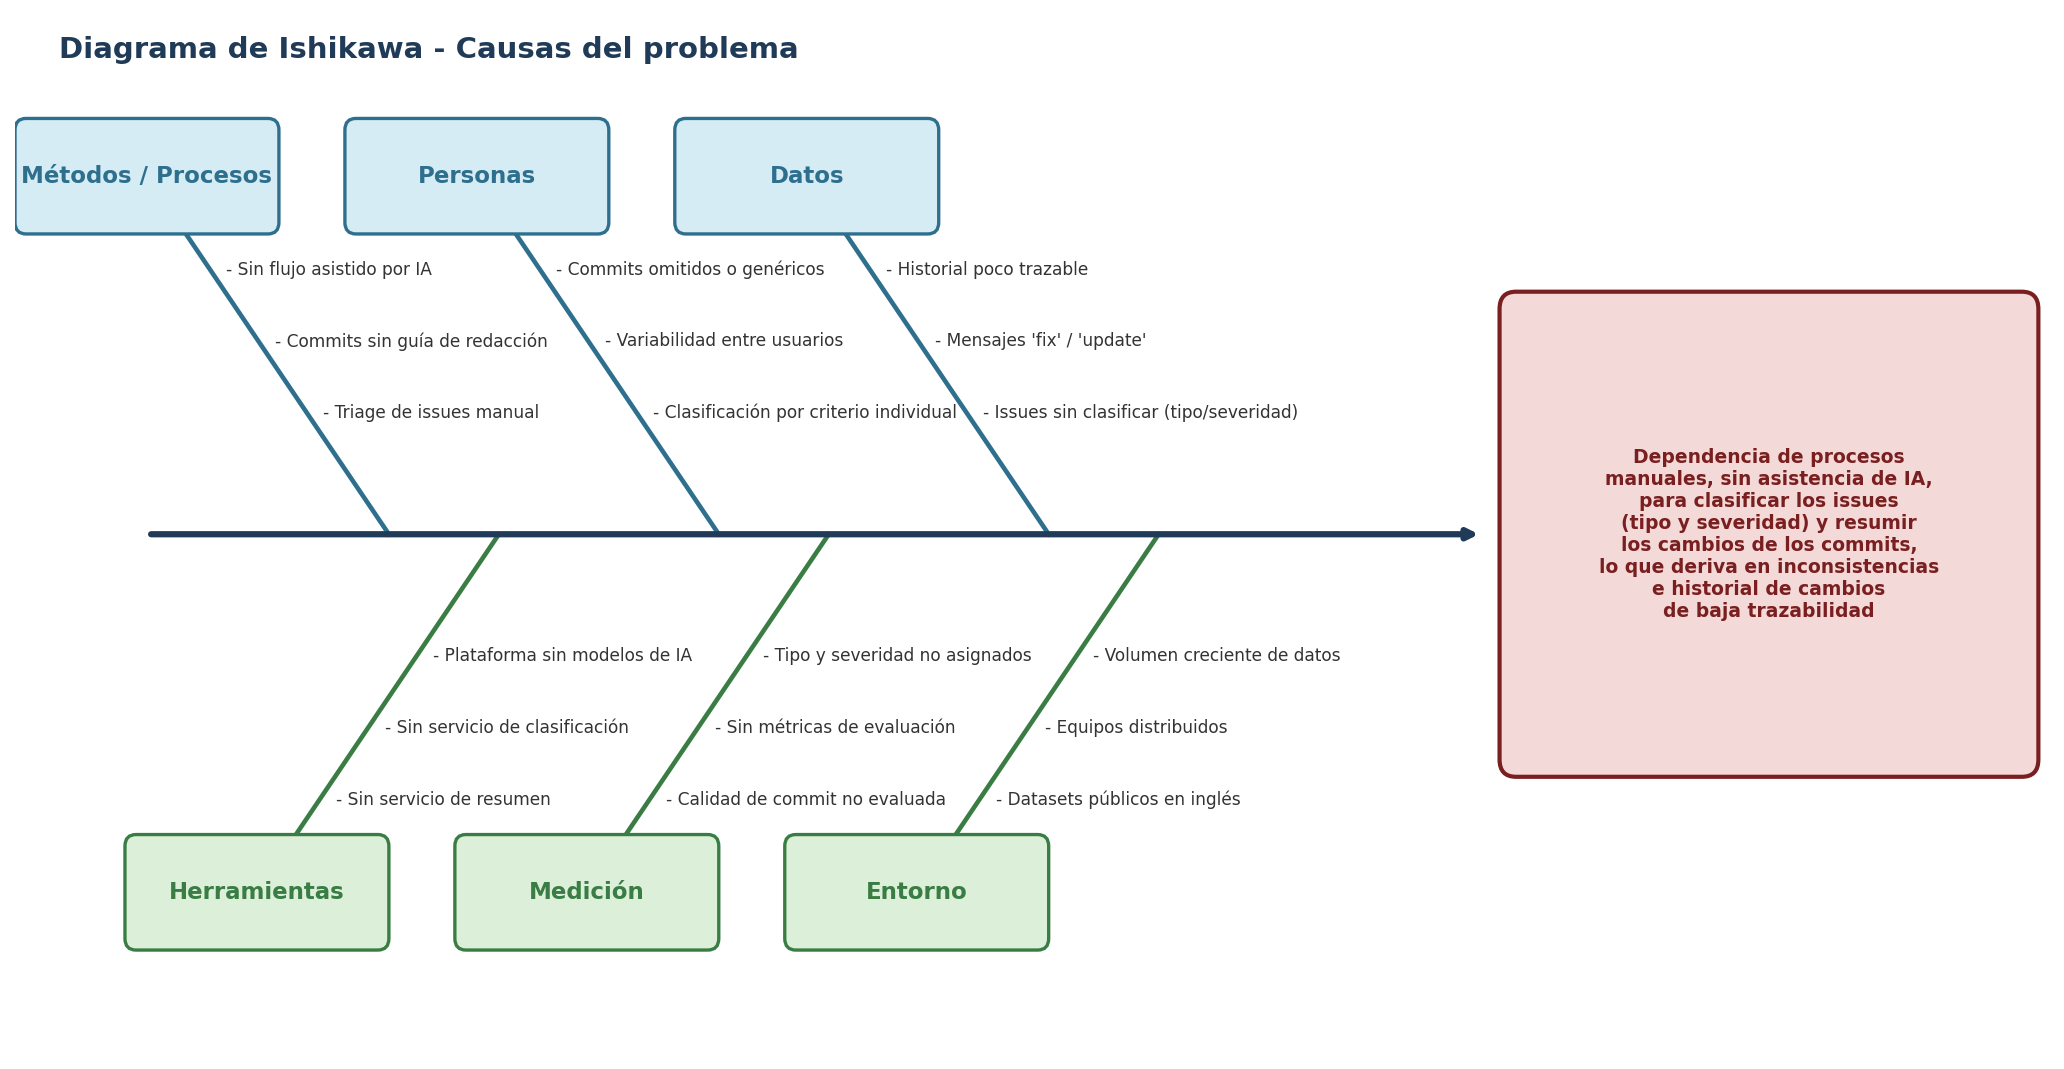
\includegraphics[width=14cm]{ishikawa_issues_commits.png}

    \centering{\textit{Nota.} Fuente: Elaboración propia, 2026}
    \label{fig:ishikawa_issues_commits}
\end{figure}

Como se visualizó en la figura anterior, la operación actual de la plataforma presenta las siguientes limitaciones:

\begin{itemize}
    \item Los \textit{issues} se crean sin clasificación automática: ni su tipo (error, mejora o pregunta) ni su nivel de severidad se asignan de forma sistemática.

    \item La clasificación y priorización (\textit{triage}) de las incidencias depende del criterio individual de cada usuario, lo que genera variabilidad en los resultados.

    \item Las incidencias críticas pueden pasar desapercibidas entre tareas de menor prioridad, retrasando su atención y resolución.

    \item Los mensajes de \textit{commit} se redactan manualmente, con calidad y nivel de detalle heterogéneos, incluyendo mensajes vacíos o genéricos (por ejemplo, ``fix'' o ``update'').

    \item La baja calidad de los mensajes de \textit{commit} dificulta la trazabilidad de los cambios y la comprensión del historial de un repositorio.

    \item La redacción de mensajes descriptivos consume tiempo del desarrollador y, con frecuencia, se omite o se posterga.

    \item La plataforma no dispone de ningún mecanismo asistido por \acrshort{IA} que apoye al usuario en la clasificación de los \textit{issues} ni en el resumen de los cambios de los \textit{commits}.
\end{itemize}

Por estos motivos, un mismo escenario puede recibir clasificaciones distintas según el usuario que lo gestione, y el historial de cambios pierde valor como fuente de trazabilidad del proyecto.

\paragraph{Problema central}

Como resultado de la situación descrita anteriormente, se identifica el siguiente problema central:

\begin{quote}
\textbf{Dependencia de procesos manuales, sin asistencia de inteligencia artificial, para clasificar el tipo y la severidad de los \textit{issues} y resumir los cambios de los \textit{commits} en la plataforma Mini-GitHub, lo que deriva en inconsistencias y en un historial de cambios de baja trazabilidad.}
\end{quote}

Esta situación genera demoras en la priorización de incidencias relevantes, inconsistencias en su clasificación y una pérdida progresiva de la calidad documental del repositorio. Según \cite{Lamkanfi2010}, la severidad de un reporte puede inferirse de su contenido textual, lo que evidencia que la clasificación manual desaprovecha información ya presente en los datos. De manera análoga, \cite{Jiang2017} señalan que la redacción manual de mensajes de \textit{commit} es una tarea repetitiva y frecuentemente descuidada, pese a su importancia para el mantenimiento del software. En ausencia de modelos que asistan estas tareas, el proceso permanece sujeto al criterio individual y susceptible de inconsistencias entre usuarios.

\paragraph{Formulación de la pregunta problema}

¿Cómo se pueden incorporar modelos de aprendizaje automático, entrenados por el equipo a partir de conjuntos de datos públicos, en la plataforma Mini-GitHub para asistir a los usuarios en la clasificación automática del tipo y la severidad de los \textit{issues} y en el resumen de los cambios de los \textit{commits}, de manera integrada con los microservicios existentes?


\subsection{Objetivos}

Dentro del presente trabajo se persiguen los siguientes objetivos.

\subsubsection{Objetivo general}

Desarrollar e integrar dos modelos de aprendizaje automático en la plataforma Mini-GitHub —un clasificador del tipo y la severidad de los \textit{issues} y un modelo de resumen automático de los cambios de los \textit{commits}—, entrenados por el equipo a partir de conjuntos de datos públicos, para asistir a los usuarios en el \textit{triage} de incidencias y en la documentación de los cambios de código, validando su funcionamiento con datos reales de la plataforma.

\subsubsection{Objetivos específicos}

    \begin{itemize}
        \item Recolectar y preparar los conjuntos de datos de entrenamiento de \textit{issues} etiquetados por tipo y por severidad, y de pares \textit{diff}--resumen de \textit{commit}, para disponer de datos consistentes que alimenten ambos modelos, mediante análisis exploratorio, limpieza, tokenización y particionamiento en subconjuntos de entrenamiento, validación y prueba.

        \item Entrenar y validar el modelo de clasificación de \textit{issues}, para asignar automáticamente a cada incidencia su tipo (error, mejora o pregunta) y su nivel de severidad, mediante vectorización del texto (\textit{Term Frequency--Inverse Document Frequency}) y algoritmos de aprendizaje automático supervisado, evaluando su desempeño con la métrica F1-score macro.

        \item Entrenar y validar el modelo de resumen de \textit{commits}, para producir un resumen en lenguaje natural a partir de los cambios de código (\textit{diff}), mediante un modelo secuencia a secuencia de aprendizaje profundo, evaluando su desempeño con las métricas BLEU y ROUGE.

        \item Integrar ambos modelos como microservicios \acrshort{REST} en la arquitectura de Mini-GitHub, para que sus predicciones sean consumidas por los servicios de \textit{issues} y de archivos, validando su funcionamiento mediante pruebas con datos reales de la plataforma.
    \end{itemize}


\subsection{Justificación}

El desarrollo del presente proyecto se justifica desde cuatro perspectivas fundamentales que sustentan su pertinencia y valor.

\subsubsection{Justificación técnica}

Desde el punto de vista técnico, el proyecto integrará en una arquitectura de microservicios dos modelos de aprendizaje automático expuestos como servicios independientes mediante \acrshort{API} \acrshort{REST}, manteniendo el bajo acoplamiento característico del sistema. El desarrollo abarcará múltiples áreas de la ingeniería de software y de la ciencia de datos: la preparación y el procesamiento de datos textuales, la aplicación de técnicas de \acrshort{ML} y de \acrfull{PLN}, el entrenamiento de modelos de aprendizaje supervisado y de aprendizaje profundo, y la construcción de servicios de inferencia con \textit{FastAPI} y su contenerización con Docker. Adicionalmente, el proyecto aplicará prácticas básicas de \acrfull{MLOps}, como el versionado de los artefactos del modelo y su despliegue reproducible, alineando el componente de inteligencia artificial con el enfoque de \textit{DevOps} del módulo.

\subsubsection{Justificación operativa}

A nivel operativo, el proyecto responderá a limitaciones concretas en el uso de la plataforma Mini-GitHub. La clasificación automática del tipo y la severidad reducirá el esfuerzo manual de \textit{triage} y mejorará la priorización de las incidencias, mientras que el resumen automático de los cambios de los \textit{commits} reducirá el esfuerzo de redacción y elevará la calidad y consistencia del historial de cambios. En conjunto, ambas capacidades mejorarán la experiencia del usuario y la trazabilidad de los proyectos alojados en la plataforma.

\subsubsection{Justificación académica}

Desde la perspectiva académica, el proyecto contribuirá a la formación profesional al integrar, en un caso de aplicación real, los conocimientos del módulo de \textit{DevOps e Inteligencia Artificial}: la construcción de modelos de \acrshort{ML} como producto, su evaluación rigurosa mediante métricas estándar y su despliegue e integración en una arquitectura de software existente. Asimismo, el proyecto generará documentación técnica que podrá servir como referencia para futuros desarrollos similares.

\subsubsection{Justificación metodológica}

En términos metodológicos, el proyecto adoptará el marco \textit{CRISP-DM} (\textit{Cross-Industry Standard Process for Data Mining}) para guiar el ciclo de vida de los modelos —comprensión del problema y de los datos, preparación, modelado, evaluación y despliegue—, complementado con entregas incrementales que permitirán validar avances de forma continua. Este enfoque garantizará que el desarrollo de los modelos siga un proceso sistemático, reproducible y orientado a la evaluación objetiva de los resultados.


\subsection{Alcances}

\begin{itemize}
  \item El proyecto contemplará el desarrollo de dos modelos: (1) un clasificador de \textit{issues} por tipo (error, mejora o pregunta) y por severidad (crítica, alta, media o baja), y (2) un modelo de resumen automático de los cambios de un \textit{commit} a partir de su \textit{diff}.

  \item El entrenamiento de ambos modelos se realizará de forma \textit{offline} a partir de conjuntos de datos públicos, externos al entorno de producción de la plataforma.

  \item Cada modelo se empaquetará y desplegará como un microservicio de inferencia mediante \textit{FastAPI} y Docker, exponiendo sus capacidades a través de \acrshort{API} \acrshort{REST} documentadas.

  \item Los modelos se integrarán con los microservicios de \textit{issues} y de archivos de Mini-GitHub, persistiendo los resultados relevantes (por ejemplo, el tipo y la severidad estimados de cada incidencia).

  \item El desempeño de los modelos se evaluará con métricas estándar: F1-score macro para la clasificación, y BLEU y ROUGE para el resumen de texto.

  \item La validación final se realizará en el entorno de la plataforma, contrastando las predicciones de los modelos con datos reales de \textit{issues} y \textit{commits}.

  \item El procesamiento se centrará en el contenido textual: título y descripción de los \textit{issues}, y representación textual de los \textit{diffs} de los \textit{commits}.
\end{itemize}

\subsection{Límites}

\begin{itemize}
  \item Los modelos serán entrenados por el equipo como producto final del proyecto; no se emplearán modelos de lenguaje de gran escala (\textit{Large Language Models}) de terceros mediante servicios externos de propósito general.

  \item El modelo de resumen se limitará a los cambios de un \textit{commit} individual; no abarcará el resumen de varios \textit{commits}, la generación de descripciones completas de \textit{pull requests} ni la generación de código.

  \item El sistema funcionará como herramienta de asistencia: las sugerencias de tipo, severidad y resumen podrán ser aceptadas o modificadas por el usuario, recayendo la decisión final en su criterio.

  \item No se implementará un sistema de reentrenamiento automático y continuo en producción; el reentrenamiento de los modelos se realizará de forma manual y periódica.

  \item El proyecto no abordará otras funcionalidades de inteligencia artificial fuera de las dos descritas (por ejemplo, búsqueda semántica, recomendación de repositorios o detección de duplicados).

  \item El procesamiento se limitará a contenido textual; no contemplará el análisis de archivos binarios, imágenes ni recursos no textuales.

  \item Los textos se procesarán principalmente en idioma inglés, en concordancia con los conjuntos de datos públicos utilizados.

  \item No se realizará evaluación económica ni estudio de retorno de inversión del desarrollo.
\end{itemize}


\begin{comment}
% ---------------------------------------------------------------------------
% ENTRADAS .bib SUGERIDAS PARA LAS CITAS UTILIZADAS EN ESTE CAPÍTULO
% (verificar/ajustar datos antes de la entrega; las URLs fueron confirmadas)
% ---------------------------------------------------------------------------
@inproceedings{Kallis2019,
  author    = {Kallis, Rafael and Di Sorbo, Andrea and Canfora, Gerardo and Panichella, Sebastiano},
  title     = {Ticket Tagger: Machine Learning Driven Issue Classification},
  booktitle = {IEEE International Conference on Software Maintenance and Evolution (ICSME)},
  year      = {2019}
}

@inproceedings{Lamkanfi2010,
  author    = {Lamkanfi, Ahmed and Demeyer, Serge and Giger, Emanuel and Goethals, Bart},
  title     = {Predicting the Severity of a Reported Bug},
  booktitle = {7th IEEE Working Conference on Mining Software Repositories (MSR)},
  year      = {2010}
}

@inproceedings{Jiang2017,
  author    = {Jiang, Siyuan and Armaly, Ameer and McMillan, Collin},
  title     = {Automatically Generating Commit Messages from Diffs using Neural Machine Translation},
  booktitle = {32nd IEEE/ACM International Conference on Automated Software Engineering (ASE)},
  year      = {2017}
}

@inproceedings{See2017,
  author    = {See, Abigail and Liu, Peter J. and Manning, Christopher D.},
  title     = {Get To The Point: Summarization with Pointer-Generator Networks},
  booktitle = {55th Annual Meeting of the Association for Computational Linguistics (ACL)},
  year      = {2017}
}

@inproceedings{Liu2019,
  author    = {Liu, Zhongxin and Xia, Xin and Treude, Christoph and Lo, David and Li, Shanping},
  title     = {Automatic Generation of Pull Request Descriptions},
  booktitle = {34th IEEE/ACM International Conference on Automated Software Engineering (ASE)},
  year      = {2019},
  note      = {arXiv:1909.06987}
}

@misc{NLBSE2024,
  author       = {{NLBSE}},
  title        = {{NLBSE'24} Tool Competition on Issue Report Classification},
  year         = {2024},
  howpublished = {\url{https://github.com/nlbse2024/issue-report-classification}}
}

@misc{Anthropic2026,
  author       = {{Anthropic}},
  title        = {Claude (Opus 4.8) [Modelo de lenguaje extenso]},
  year         = {2026},
  howpublished = {\url{https://claude.ai}}
}
% ---------------------------------------------------------------------------
\end{comment}

    % No modificar estas líneas de código, por favor dirigirse a MARCO PRÁCTICO
%
% NOTA: capítulo reescrito para el proyecto "DevOps e IA - Mini-GitHub".
%   Figuras en la misma carpeta: fig_arquitectura.png, fig_flujo_resumidor.png,
%   fig_pipeline_mlops.png, fig_despliegue_ecs.png (generadas con gen_figuras_diagramas.py).
%   Detalle extenso (código, tablas completas) -> Anexos.
%
\newpage

%------------------------
%
%       MARCO PRÁCTICO
%
%------------------------

\section{MARCO PRÁCTICO}

En este capítulo se documenta la ingeniería del proyecto: la propuesta de solución, los requerimientos, la arquitectura, el desarrollo de los dos modelos de aprendizaje automático, su encapsulamiento como microservicios de inferencia, la automatización del ciclo de vida (\acrshort{MLOps}), la integración con la plataforma y el despliegue en la nube. La construcción siguió el marco \acrshort{CRISPDM}, coherente con lo comprometido en la introducción.

\subsection{Propuesta de solución}

\textbf{Tema:} \textit{``Incorporación de dos modelos de aprendizaje automático —clasificación de \textit{issues} y resumen de \textit{commits}— en la plataforma de microservicios Mini-GitHub''}.

\vspace{0.4em}

Se propuso dotar a la plataforma Mini-GitHub de dos capacidades asistidas por \acrfull{IA}, entrenadas por el equipo a partir de conjuntos de datos públicos y sin emplear modelos de lenguaje de gran escala de terceros. La primera, un clasificador que, a partir del título y la descripción de un \textit{issue}, sugiere su \textbf{tipo} (\textit{bug}, \textit{feature} o \textit{question}) y su \textbf{severidad} (crítica, alta, media o baja). La segunda, un modelo generativo que produce un \textbf{resumen} en lenguaje natural del cambio de código (\textit{diff}) de un \textit{commit}. Ambas capacidades se exponen como microservicios \acrshort{REST} independientes, se integran en el frontend como sugerencias editables y se despliegan en la nube junto al resto de la plataforma.

\subsection{Requerimientos}

\subsubsection{Requerimientos funcionales (RF)}
\begin{itemize}\itemsep=1pt
    \item \textbf{RF1:} El sistema clasifica un \textit{issue} por tipo y por severidad a partir de su texto.
    \item \textbf{RF2:} El sistema genera un resumen del cambio de un \textit{commit} a partir de su \textit{diff}.
    \item \textbf{RF3:} Ambos modelos se exponen mediante \acrshort{API} \acrshort{REST} documentadas con autenticación por \textit{token} JWT.
    \item \textbf{RF4:} El frontend consume ambas capacidades como sugerencias que el usuario puede aceptar o modificar.
    \item \textbf{RF5:} El ciclo de entrenamiento, evaluación y despliegue de los modelos se automatiza mediante un orquestador.
\end{itemize}

\subsubsection{Requerimientos no funcionales (RNF)}
\begin{itemize}\itemsep=1pt
    \item \textbf{RNF1:} Los modelos se entrenan por el equipo, sin modelos preentrenados de terceros (restricción académica del proyecto).
    \item \textbf{RNF2:} La inferencia se ejecuta en \acrshort{CPU} (restricción de despliegue), con modelos ligeros.
    \item \textbf{RNF3:} El desempeño se mide con métricas estándar: \textbf{F1-score macro} (clasificación) y \acrshort{BLEU}/\acrshort{ROUGE} (resumen).
    \item \textbf{RNF4:} Cada modelo se conteneriza (Docker) y se despliega de forma reproducible.
    \item \textbf{RNF5:} La solución mantiene el bajo acoplamiento de la arquitectura de microservicios existente.
\end{itemize}

\subsection{Arquitectura de la solución}

La solución se incorpora a la arquitectura de microservicios de Mini-GitHub como dos servicios nuevos, sin alterar los servicios de negocio existentes. Como se observa en la Figura~\ref{fig:arquitectura}, el frontend (Next.js) es el punto de entrada del usuario y, autenticado mediante Keycloak (JWT), consume tanto los microservicios de negocio (Java/Spring) como los dos \textbf{servicios de \acrshort{IA}} (Python/FastAPI): el clasificador de \textit{issues} y el resumidor de \textit{commits}. Este diseño preserva la separación de responsabilidades: los modelos son piezas desacopladas que se comunican por contratos \acrshort{REST} tipados.

\begin{figure}[H]
    \centering
    \caption{Arquitectura de la plataforma con los dos servicios de IA incorporados.}
    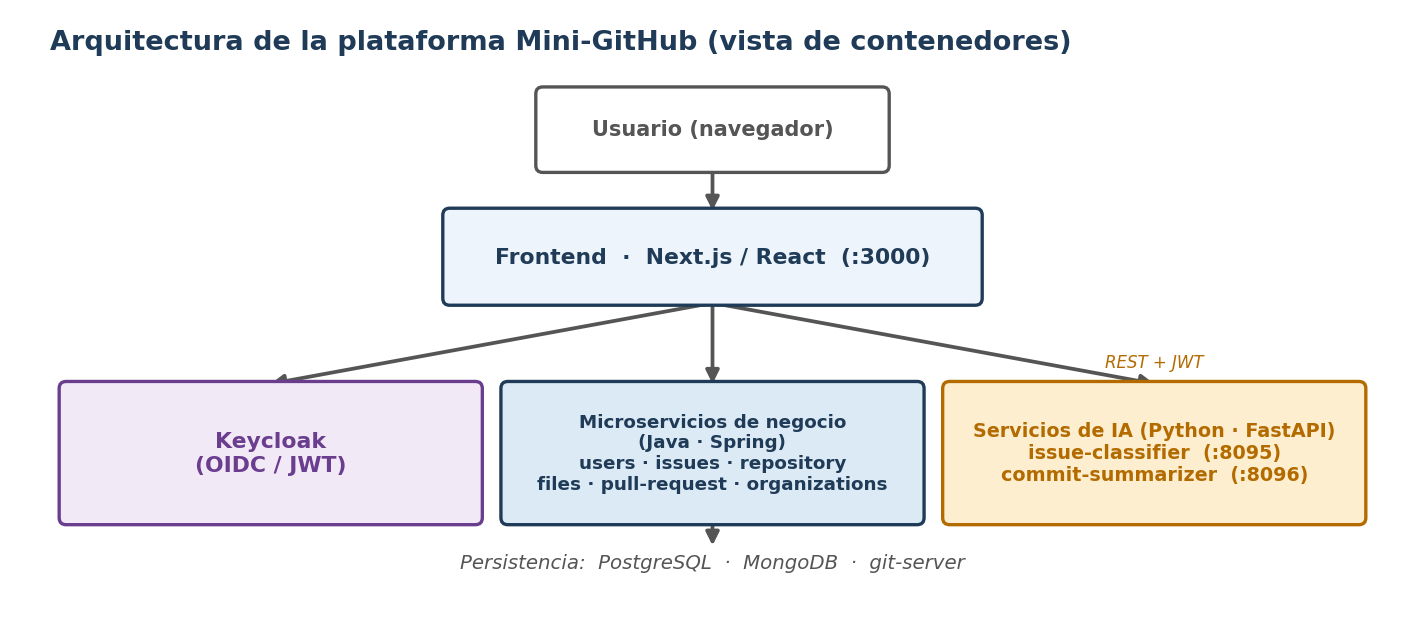
\includegraphics[width=14cm]{fig_arquitectura.png}

    \centering{\textit{Nota.} Fuente: Elaboración propia, 2026}
    \label{fig:arquitectura}
\end{figure}

\subsection{Modelo 1 — Clasificación de \textit{issues} (tipo y severidad)}

\textbf{Conjuntos de datos.} El clasificador de tipo se entrenó con el dataset \textit{GitHub Bugs Prediction} (Kaggle), $\sim$150.000 \textit{issues} reales con título, cuerpo y etiqueta (\textit{bug}/\textit{feature}/\textit{question}). El de severidad se entrenó con el \textit{Eclipse and Mozilla Defect Tracking Dataset} \citep{Lamkanfi2010} (214.903 reportes), aplicando un mapeo de las severidades de Bugzilla a los cuatro niveles del proyecto (\textit{blocker}/\textit{critical}$\rightarrow$crítica, \textit{major}$\rightarrow$alta, \textit{normal}$\rightarrow$media, \textit{minor}/\textit{trivial}$\rightarrow$baja).

\textbf{Preparación.} Se concatenaron título y cuerpo; la limpieza reemplaza bloques de código por el token \texttt{CODE} y las \acrshort{URL}s por \texttt{URL} —preservando su \textit{presencia} como señal sin el ruido léxico—, elimina \acrshort{HTML} y normaliza a minúsculas. La partición fue estratificada 80/10/10 con semilla 42.

\textbf{Modelado.} Se empleó vectorización \acrfull{TFIDF} (100.000 rasgos, unigramas y bigramas) y se comparó \textit{Regresión Logística} frente a \textit{Support Vector Machine} lineal, ambos con \texttt{class\_weight=balanced} para atenuar el desbalance de clases, seleccionando el de mayor F1-score macro en validación. Los modelos lineales sobre \acrshort{TFIDF} constituyen un \textit{baseline} fuerte, rápido y apto para inferencia en \acrshort{CPU}. El resultado es un \textit{pipeline} de \textit{scikit-learn} (vectorizador + clasificador) serializado como artefacto \texttt{.joblib}. Los resultados cuantitativos se presentan en el Capítulo de Análisis de Resultados.

\subsection{Modelo 2 — Resumen de \textit{commits} (\textit{diff} $\rightarrow$ mensaje)}

\textbf{Conjunto de datos.} Se utilizó el corpus limpio de \textbf{NNGen} (Liu et al., 2018), derivado del corpus de \cite{Jiang2017}, con pares \textit{diff}$\rightarrow$mensaje de los 1.000 proyectos Java más populares de GitHub ($\sim$22.000 pares), ampliado con pares de Python, JavaScript, C++ y C\# del dataset \textit{MCMD} para un modelo multilenguaje.

\textbf{Arquitectura.} Se entrenó \textbf{desde cero} un modelo secuencia a secuencia ($\sim$35 millones de parámetros en su versión multilenguaje desplegada): codificador \textit{GRU} bidireccional, decodificador con \textbf{atención de Luong} y un mecanismo \textit{pointer-generator} \citep{See2017} que permite \textbf{copiar identificadores} del \textit{diff} (nombres de métodos, versiones) al mensaje, superando la debilidad del seq2seq base ante vocabulario fuera de rango. Corresponde a la línea de \acrfull{NMT} aplicada a mensajes de \textit{commit}.

\textbf{Sistema híbrido de inferencia.} El servicio no delega la respuesta únicamente a la red neuronal: implementa una cascada de cuatro niveles (Figura~\ref{fig:flujoresumidor}) que responde con el primer nivel cuya condición se cumple: (1) heurísticas de ingeniería de software (línea ChangeScribe) que extraen patrones verificables del propio \textit{diff}; (2) recuperación estilo NNGen cuando existe un \textit{diff} vecino suficientemente similar; (3) el modelo generativo \textit{pointer-generator} con \textit{beam search}; y (4) un respaldo por nombres de archivo. Esta estrategia prioriza la información verificable del cambio y mejora la robustez sobre \textit{diffs} fuera de distribución.

\begin{figure}[H]
    \centering
    \caption{Sistema híbrido en cascada del resumidor de \textit{commits}.}
    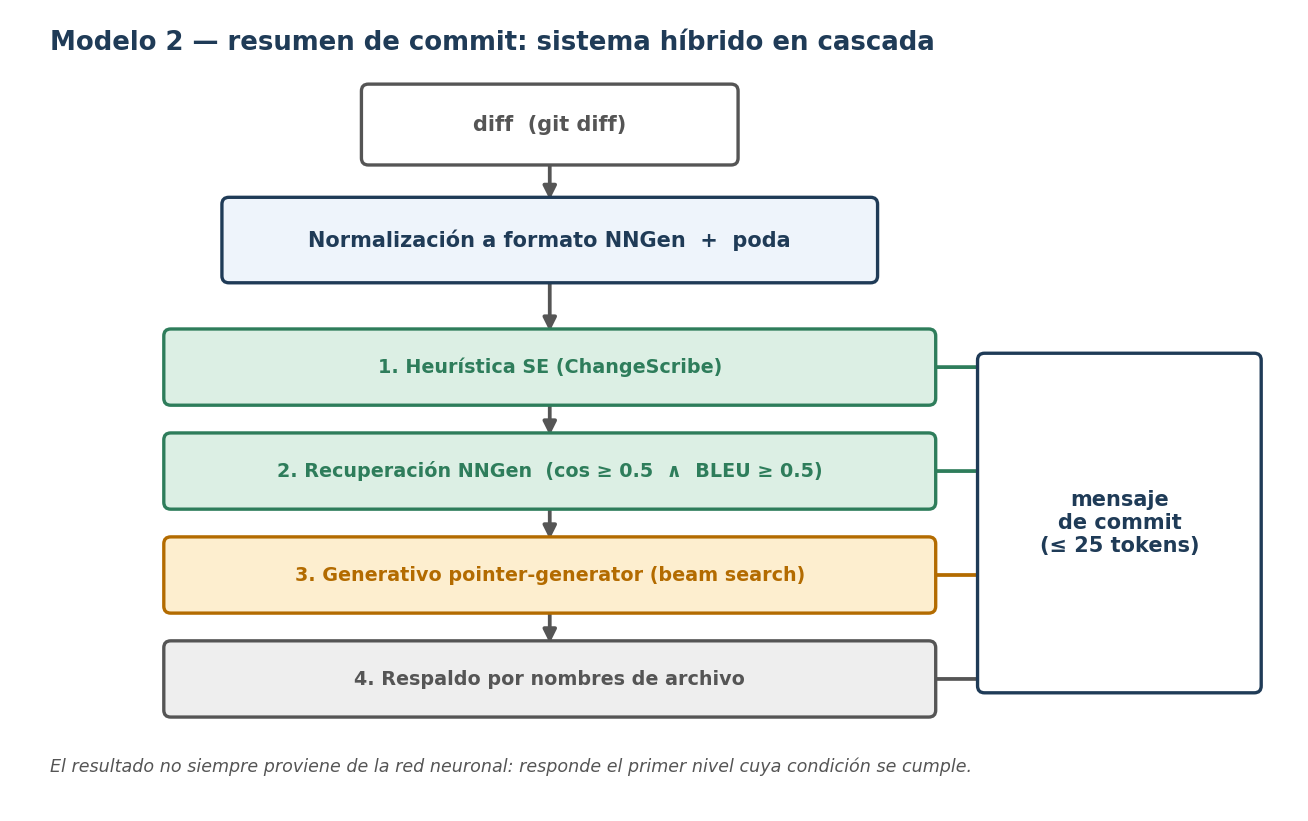
\includegraphics[width=13cm]{fig_flujo_resumidor.png}

    \centering{\textit{Nota.} Fuente: Elaboración propia, 2026}
    \label{fig:flujoresumidor}
\end{figure}

\subsection{Microservicios de inferencia}

Cada modelo se encapsula en un microservicio \textit{FastAPI} independiente, contenerizado con Docker y protegido con validación de \textit{token} JWT contra Keycloak, replicando el patrón de seguridad de los microservicios de negocio. El modelo viaja \textbf{dentro de la imagen}, de modo que cada versión de imagen queda ligada a una versión exacta del modelo (\acrshort{MLOps} básico). Los contratos se resumen en la Tabla~\ref{tab:endpoints_ia}.

\begin{table}[H]
\centering
\caption{Contratos REST de los servicios de IA}
{\small
\begin{tabular}{|l|c|l|p{4.6cm}|}
\hline
\textbf{Servicio} & \textbf{Puerto} & \textbf{Endpoint} & \textbf{Entrada $\rightarrow$ Salida} \\
\hline
issue-classifier & 8095 & \texttt{POST /v1/classify} & \texttt{\{title, body\}} $\rightarrow$ \texttt{\{tipo, severidad, confianza\}} \\
\hline
commit-summarizer & 8096 & \texttt{POST /v1/summarize} & \texttt{\{diff\}} $\rightarrow$ \texttt{\{resumen\}} \\
\hline
\end{tabular}
}

\centering{\textit{Nota.} Fuente: Elaboración propia, 2026}
\label{tab:endpoints_ia}
\end{table}

\subsection{Automatización del ciclo de vida (\acrshort{MLOps})}

El ciclo de vida de los modelos se automatizó con un orquestador \textit{Apache Airflow}. Los tres modelos (tipo, severidad y resumidor) comparten un mismo grafo de tareas, parametrizado por una fábrica de \textit{DAG}. Como ilustra la Figura~\ref{fig:pipelinemlops}, el flujo encadena \texttt{preprocess} $\rightarrow$ \texttt{train} $\rightarrow$ \texttt{evaluate} y, mediante una \textbf{compuerta de calidad} (\textit{quality gate}), sólo registra y despliega el modelo si supera un umbral configurable (F1-score macro para la clasificación, \acrshort{BLEU} para el resumen); en caso contrario lo rechaza. El registro versiona cada modelo y el despliegue se realiza por \textit{hot-swap} (recarga en caliente del servicio, sin reinicio).

\begin{figure}[H]
    \centering
    \caption{Pipeline MLOps con compuerta de calidad, registro y despliegue en caliente.}
    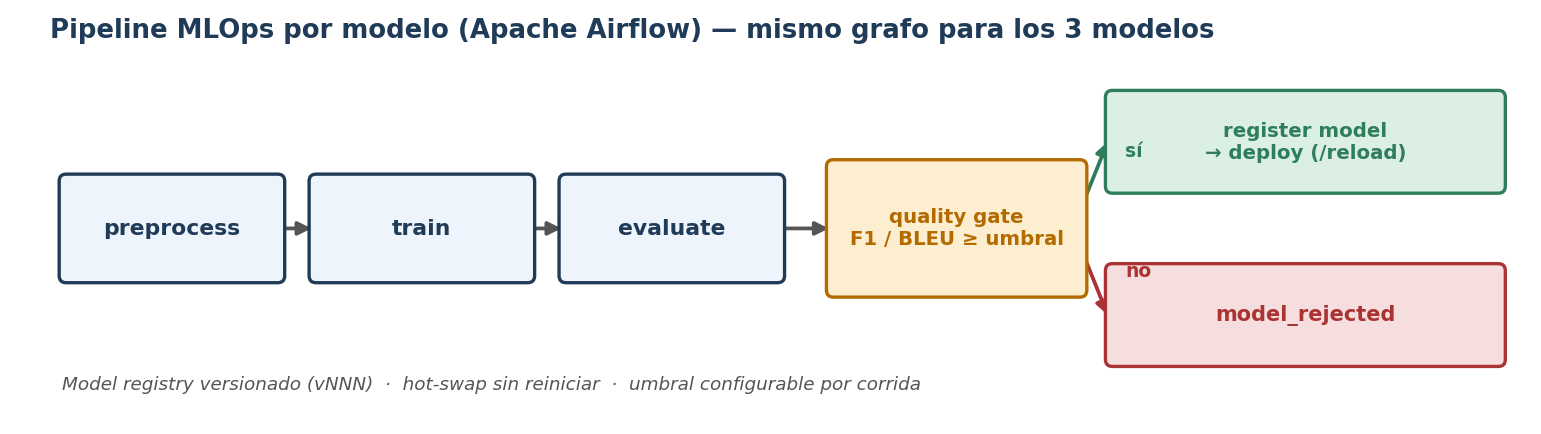
\includegraphics[width=15cm]{fig_pipeline_mlops.png}

    \centering{\textit{Nota.} Fuente: Elaboración propia, 2026}
    \label{fig:pipelinemlops}
\end{figure}

\subsection{Integración con la plataforma}

La integración con el frontend se implementó mediante una capa de servicio (\texttt{ai.ts}) que enruta las peticiones a ambos modelos y adjunta el \textit{token} del usuario. En el formulario de creación de \textit{issue}, un botón \textit{``Sugerir tipo y severidad''} invoca al clasificador y muestra el tipo (con su nivel de confianza) y la severidad como etiquetas de color; el usuario puede \textbf{aplicarlas como \textit{labels} editables}. En el editor de archivos, un botón \textit{``Sugerir mensaje''} construye el \textit{diff}, invoca al resumidor y rellena el campo del mensaje de \textit{commit}, que el usuario puede ajustar antes de confirmar. En ambos casos la \acrshort{IA} actúa como asistencia y la decisión final es del usuario.

\subsection{Despliegue en la nube}

La plataforma completa se despliega en \textbf{AWS ECS Fargate} mediante infraestructura como código (AWS CDK). Como muestra la Figura~\ref{fig:despliegueecs}, un único \textit{stack} provisiona la red (VPC), el \textit{cluster} \texttt{github-ecs}, la base de datos gestionada (RDS PostgreSQL), el descubrimiento de servicios (Cloud Map) y los balanceadores (ALB) que exponen el frontend y las \acrshort{API}s. Los once servicios corren como tareas Fargate; los dos servicios de \acrshort{IA} se publican desde \textbf{ECR} y son consumidos internamente por el frontend. Complementariamente, cada microservicio de \acrshort{IA} incorpora un flujo de integración y entrega continua (GitHub Actions) que, ante un cambio en la rama principal, construye la imagen, la publica en ECR y actualiza el servicio en ECS.

\begin{figure}[H]
    \centering
    \caption{Despliegue de la plataforma en AWS ECS Fargate (CDK).}
    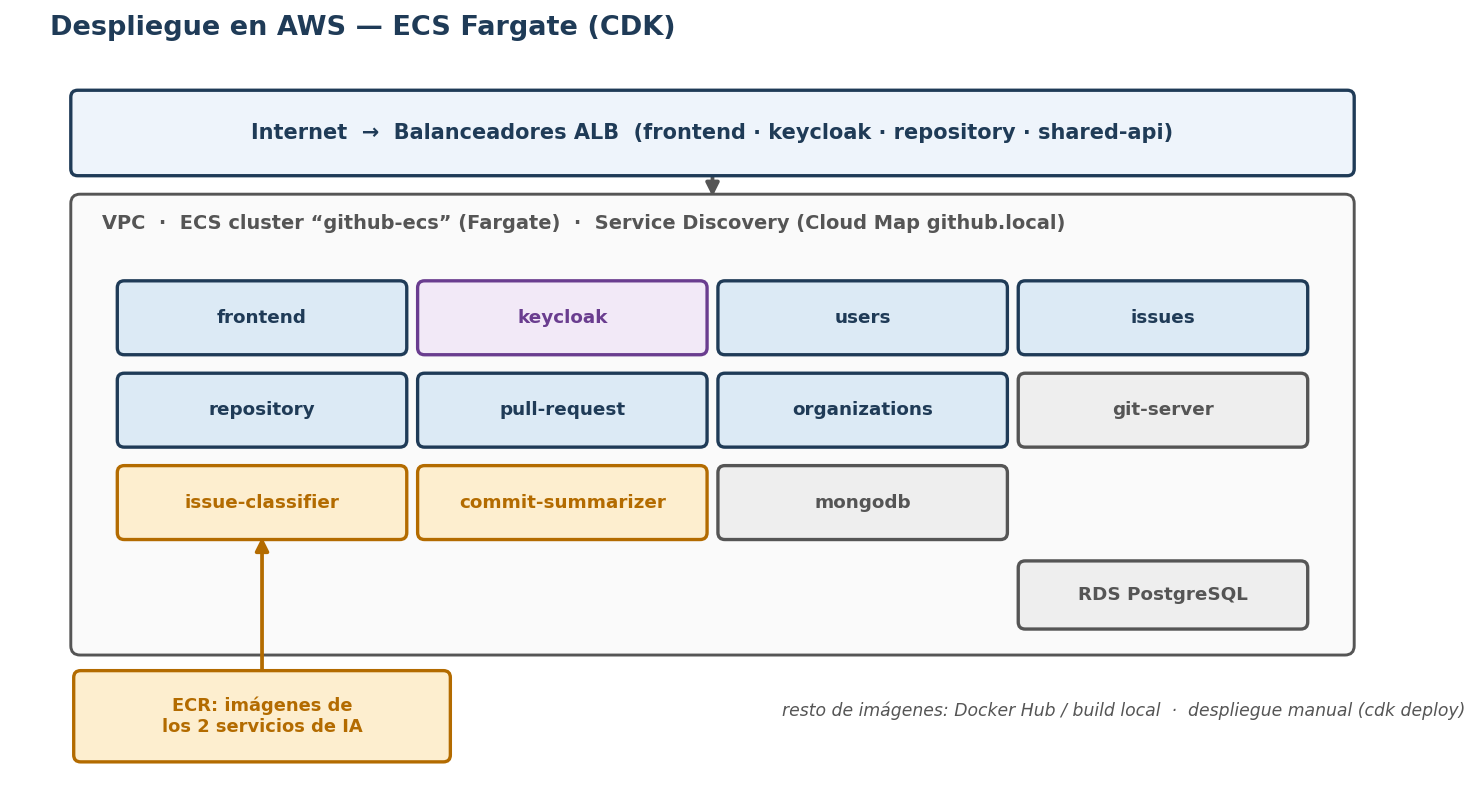
\includegraphics[width=15cm]{fig_despliegue_ecs.png}

    \centering{\textit{Nota.} Fuente: Elaboración propia, 2026}
    \label{fig:despliegueecs}
\end{figure}

\subsection{Metodología aplicada}

El desarrollo siguió el marco \acrfull{CRISPDM}: (i) \textit{comprensión del problema}, alineada con los objetivos de la introducción; (ii) \textit{comprensión y preparación de los datos}, con el análisis exploratorio, la limpieza y el particionamiento descritos; (iii) \textit{modelado}, con la selección de algoritmos por validación; (iv) \textit{evaluación}, con métricas estándar (Capítulo de Análisis de Resultados); y (v) \textit{despliegue}, materializado en los microservicios, el pipeline \acrshort{MLOps} y la infraestructura en la nube. El detalle de implementación (código, notebooks y tablas completas) se documenta en los apéndices.

    % No modificar estas líneas de código, por favor dirigirse a ANÁLISIS DE RESULTADOS
%
% NOTA: capítulo reescrito para "DevOps e IA - Mini-GitHub".
%   Figuras (carpeta actual): fig_clasif_tipo.png, fig_clasif_severidad.png,
%   fig_distribucion_clases.png, fig_resumidor_evolucion.png, fig_resumidor_lenguaje.png
%   (generadas con gen_figuras_metricas.py, con números REALES de los ENTRENAMIENTO.md).
%   Capturas de producción pendientes -> ver PENDIENTE_IMAGENES.md.
%
\newpage

%------------------------
%
%       ANÁLISIS DE RESULTADOS
%
%------------------------

\section{ANÁLISIS DE RESULTADOS}

Este capítulo presenta los resultados de la evaluación de los dos modelos, el cumplimiento de los requerimientos y la validación del sistema desplegado en producción. Las métricas se obtuvieron sobre el conjunto de prueba (evaluado una única vez, tras la selección por validación) con semilla fija 42 para garantizar reproducibilidad.

\subsection{Cumplimiento de requerimientos}

Los cinco requerimientos funcionales se cumplieron: el sistema clasifica \textit{issues} por tipo y severidad (RF1), genera resúmenes de \textit{commits} (RF2), expone ambos modelos como \acrshort{API} \acrshort{REST} autenticadas (RF3), los integra en el frontend como sugerencias editables (RF4) y automatiza el ciclo de entrenamiento--evaluación--despliegue con un \textit{pipeline} de Airflow (RF5). Los requerimientos no funcionales también se satisfacen: modelos entrenados por el equipo sin preentrenados de terceros (RNF1), inferencia en \acrshort{CPU} (RNF2), evaluación con métricas estándar (RNF3), contenerización reproducible (RNF4) y preservación del bajo acoplamiento (RNF5).

\subsection{Resultados del Modelo 1 — clasificación de \textit{issues}}

El clasificador de \textbf{tipo} alcanzó un \textbf{F1-score macro de 0{,}710} y una exactitud de 0{,}778 sobre el conjunto de prueba, seleccionando la Regresión Logística (0{,}711 en validación) sobre la \textit{SVM} lineal (0{,}707). Como se observa en la Figura~\ref{fig:clasiftipo}, las clases mayoritarias superan 0{,}80 de F1 (\textit{bug} 0{,}815; \textit{feature} 0{,}806), mientras que \textit{question} baja a 0{,}508 por su marcado desbalance (razón $\sim$5:1) y su solapamiento léxico con \textit{bug}. El uso de \texttt{class\_weight=balanced} prioriza el \textit{recall} de la clase minoritaria (0{,}588), comportamiento preferible para un sistema de sugerencias.

\begin{figure}[H]
    \centering
    \caption{Clasificador de tipo — precisión, \textit{recall} y F1 por clase (test).}
    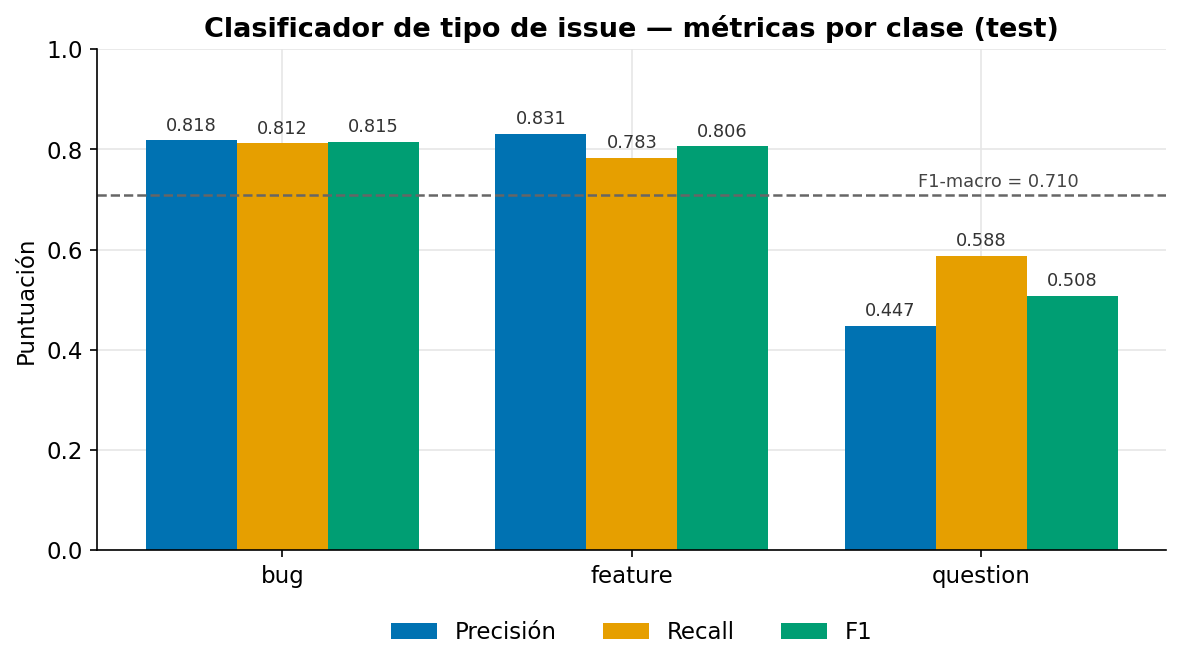
\includegraphics[width=12cm]{fig_clasif_tipo.png}

    \centering{\textit{Nota.} Fuente: Elaboración propia, 2026}
    \label{fig:clasiftipo}
\end{figure}

El clasificador de \textbf{severidad} obtuvo un \textbf{F1-score macro de 0{,}442} y exactitud 0{,}685, resultado consistente con la literatura para severidad multiclase (0{,}40--0{,}55), en línea con \cite{Lamkanfi2010}. La Figura~\ref{fig:clasifseveridad} muestra que el modelo es sólido donde más importa —detectar lo \textbf{crítico} (F1 0{,}540, \textit{recall} 0{,}579)— y en la clase mayoritaria \textit{media} (0{,}810), pero las clases \textit{alta} (0{,}225) y \textit{baja} (0{,}193) son genuinamente ambiguas, incluso para anotadores humanos. Este comportamiento se explica por el desbalance del corpus (Figura~\ref{fig:distribucion}): la clase \textit{media} (valor por defecto de Bugzilla) domina el conjunto, y la clase \textit{question} es minoritaria en el dataset de tipo. Coherentemente con el alcance del proyecto, la severidad se presenta como una \textit{sugerencia editable}.

\begin{figure}[H]
    \centering
    \caption{Clasificador de severidad — precisión, \textit{recall} y F1 por clase (test).}
    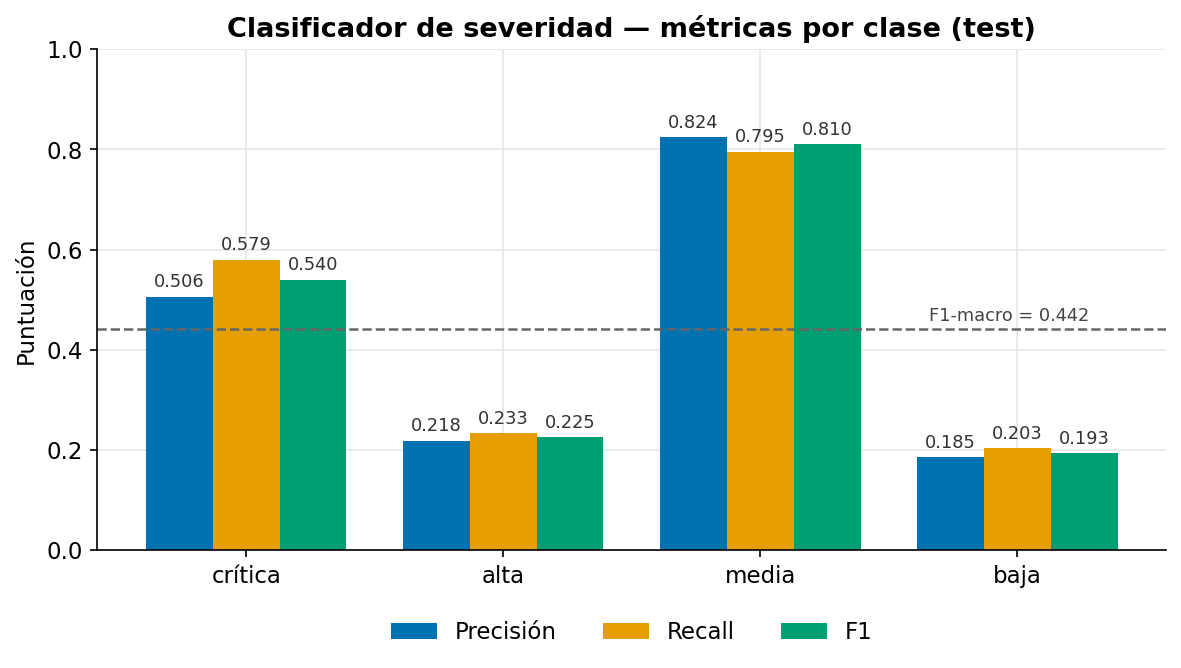
\includegraphics[width=12cm]{fig_clasif_severidad.png}

    \centering{\textit{Nota.} Fuente: Elaboración propia, 2026}
    \label{fig:clasifseveridad}
\end{figure}

\begin{figure}[H]
    \centering
    \caption{Distribución de clases en el conjunto de prueba (evidencia del desbalance).}
    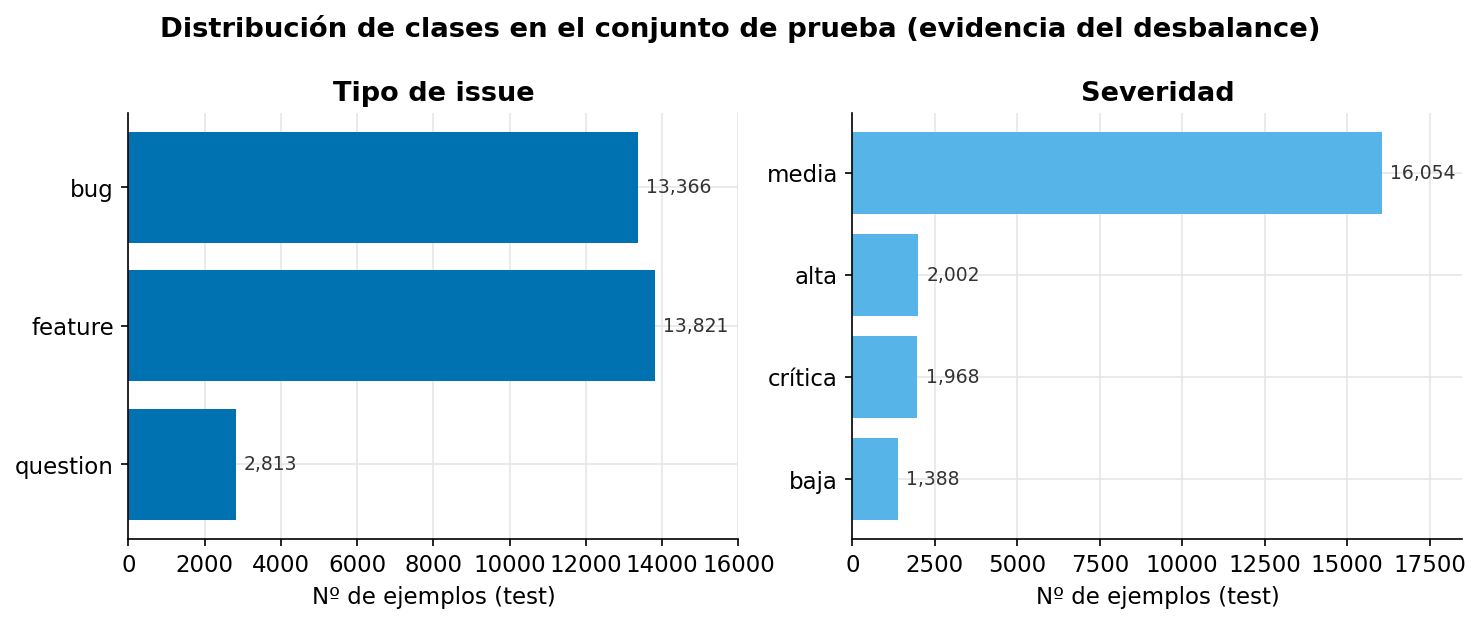
\includegraphics[width=13cm]{fig_distribucion_clases.png}

    \centering{\textit{Nota.} Fuente: Elaboración propia, 2026}
    \label{fig:distribucion}
\end{figure}

\subsection{Resultados del Modelo 2 — resumen de \textit{commits}}

El modelo generativo se evaluó con \acrshort{BLEU}-4 y \acrshort{ROUGE}-L, las métricas estándar de la tarea. La incorporación del mecanismo \textit{pointer-generator} sobre el seq2seq base produjo una mejora sustancial (Figura~\ref{fig:resumidorevolucion}): \acrshort{BLEU}-4 pasó de \textbf{6{,}68 a 11{,}62} (+74\%) y \acrshort{ROUGE}-L de \textbf{0{,}209 a 0{,}293} (+40\%), gracias a su capacidad de copiar identificadores del \textit{diff} al mensaje. La Tabla~\ref{tab:resumidor} resume esta evolución.

\begin{table}[H]
\centering
\caption{Evolución del resumidor (test, corpus Java)}
\begin{tabular}{|l|c|c|}
\hline
\textbf{Variante} & \textbf{BLEU-4} & \textbf{ROUGE-L} \\
\hline
seq2seq base & 6{,}68 & 0{,}209 \\
\textbf{pointer-generator} & \textbf{11{,}62} & \textbf{0{,}293} \\
\hline
\end{tabular}

\centering{\textit{Nota.} Fuente: Elaboración propia, 2026}
\label{tab:resumidor}
\end{table}

El modelo desplegado es la variante \textbf{multilenguaje} (v3), reentrenada desde cero sobre Java, Python, JavaScript, C++ y C\#. Alcanzó un \acrshort{BLEU}-4 \textbf{global de 11{,}79}, con desempeño homogéneo ($\sim$12) en los cuatro lenguajes nuevos (Figura~\ref{fig:resumidorlenguaje}). El \textit{trade-off} medido y aceptado fue una caída de 2{,}1 puntos en Java (9{,}52) a cambio de cobertura real en lenguajes antes fuera de dominio. Cabe notar que \acrshort{BLEU} subestima la calidad percibida en esta tarea, al comparar $n$-gramas exactos contra una única referencia en mensajes muy cortos; por ello el sistema se concibe como \textit{asistencia editable} y no como generador autónomo.

\begin{figure}[H]
    \centering
    \caption{Efecto del mecanismo de copia: BLEU-4 y ROUGE-L (seq2seq $\rightarrow$ pointer-generator).}
    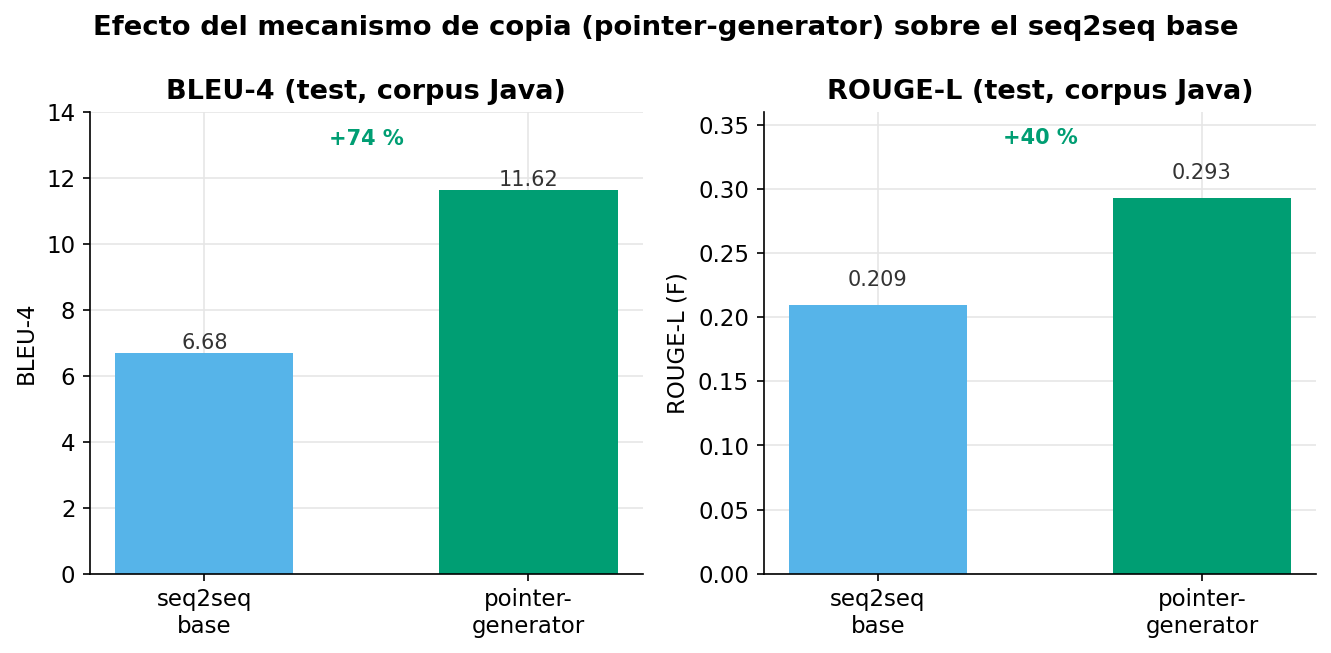
\includegraphics[width=12cm]{fig_resumidor_evolucion.png}

    \centering{\textit{Nota.} Fuente: Elaboración propia, 2026}
    \label{fig:resumidorevolucion}
\end{figure}

\begin{figure}[H]
    \centering
    \caption{BLEU-4 por lenguaje del modelo desplegado.}
    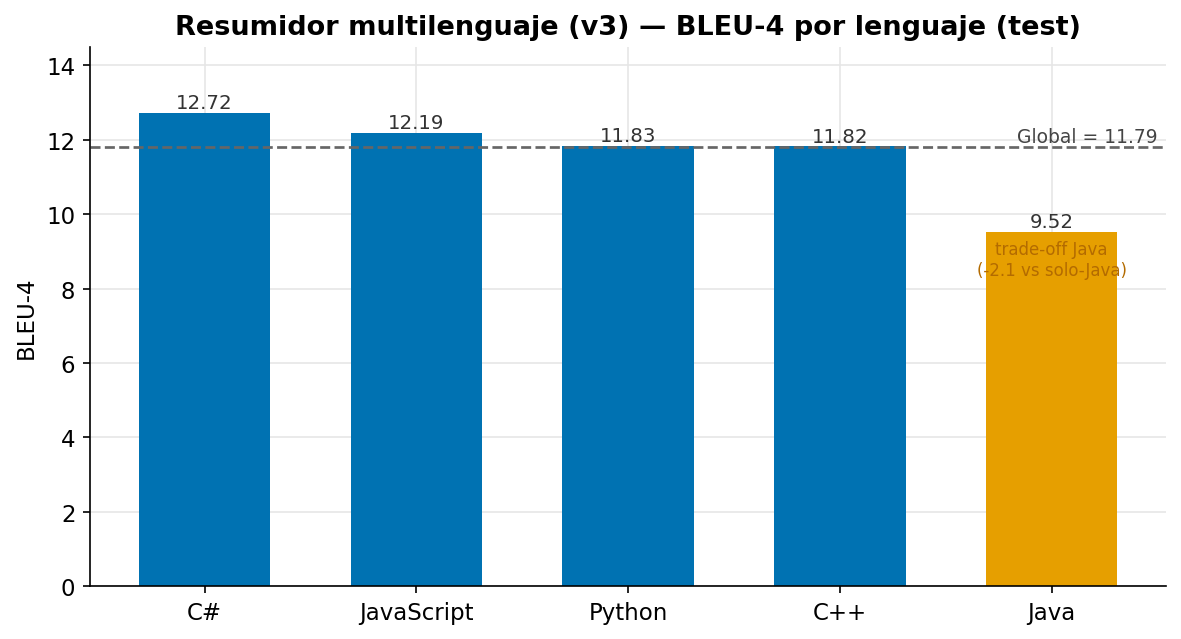
\includegraphics[width=12cm]{fig_resumidor_lenguaje.png}

    \centering{\textit{Nota.} Fuente: Elaboración propia, 2026}
    \label{fig:resumidorlenguaje}
\end{figure}

\subsection{Validación en producción}

Además de la evaluación cuantitativa sobre los conjuntos de prueba, el sistema se validó en el entorno real desplegado en AWS. Con la plataforma en producción, se ejercitaron ambos modelos sobre \textit{issues} y \textit{commits} reales de Mini-GitHub: al crear un \textit{issue}, el clasificador sugiere su tipo y severidad, que se aplican como \textit{labels} editables; y al editar un archivo, el resumidor propone el mensaje del \textit{commit}. Esta validación confirma el funcionamiento de extremo a extremo (frontend $\rightarrow$ servicios de \acrshort{IA} $\rightarrow$ persistencia) con datos reales. La evidencia gráfica de estas ejecuciones se documenta en los apéndices.

\subsection{Síntesis de resultados}

Los resultados evidencian el cumplimiento de los objetivos planteados. Los principales logros cuantificables son:

\begin{itemize}\itemsep=1pt
    \item Clasificador de tipo con \textbf{F1-macro 0{,}710} (F1 $>$ 0{,}80 en las clases mayoritarias).
    \item Clasificador de severidad con \textbf{F1-macro 0{,}442}, efectivo en la detección de lo crítico (F1 0{,}540).
    \item Resumidor con \textbf{BLEU-4 11{,}79} global (multilenguaje), tras una mejora del +74\% por el mecanismo de copia.
    \item Ambos modelos \textbf{desplegados y validados en producción}, integrados en la plataforma como asistencia editable.
\end{itemize}

Las limitaciones observadas —severidad modesta en las clases intermedias y \acrshort{BLEU} moderado del resumidor— son consistentes con la literatura y con el alcance académico del proyecto, y no comprometen el valor del sistema como herramienta de asistencia al desarrollador.

    % No modificar estas líneas de código, por favor dirigirse a CONCLUSIONES
%
% NOTA: capítulo reescrito para "DevOps e IA - Mini-GitHub".
%
\newpage
\phantomsection\addcontentsline{toc}{section}{CONCLUSIONES}

%------------------------
%
%       CONCLUSIONES
%
%------------------------

\section*{CONCLUSIONES}

El presente capítulo sintetiza los logros alcanzados durante el desarrollo e integración de los dos modelos de aprendizaje automático en la plataforma Mini-GitHub, analizando el cumplimiento de los objetivos específicos y los aprendizajes generados.

\vspace{0.5em}

\textbf{Conclusiones por objetivo específico:}

\begin{itemize}\itemsep=2pt

    \item \textbf{OE1 — Preparación de los conjuntos de datos:} Se recolectaron y prepararon los datasets públicos requeridos: \textit{GitHub Bugs Prediction} (Kaggle) para el tipo, el \textit{Eclipse and Mozilla Defect Tracking Dataset} \citep{Lamkanfi2010} para la severidad, y el corpus NNGen ampliado con MCMD para el resumen de \textit{commits}. Se aplicó análisis exploratorio, limpieza, tokenización y partición estratificada 80/10/10 con semilla 42, garantizando la reproducibilidad.

    \item \textbf{OE2 — Clasificador de \textit{issues} (tipo y severidad):} Se entrenó y validó un modelo de clasificación supervisada (\acrshort{TFIDF} + clasificador lineal), alcanzando \textbf{F1-score macro de 0{,}710} en tipo y \textbf{0{,}442} en severidad, con desempeño sólido en las clases mayoritarias y en la detección de lo crítico. El modelo se sirve en el microservicio \texttt{issue-classifier-ms}.

    \item \textbf{OE3 — Resumidor de \textit{commits}:} Se construyó desde cero un modelo secuencia a secuencia con mecanismo \textit{pointer-generator}, sin modelos preentrenados de terceros, que alcanzó un \acrshort{BLEU}-4 global de \textbf{11{,}79} en su versión multilenguaje. El mecanismo de copia mejoró el \acrshort{BLEU}-4 en un +74\% respecto al seq2seq base. El servicio complementa la red con una estrategia híbrida de heurísticas y recuperación.

    \item \textbf{OE4 — Integración en la plataforma:} Ambos modelos se encapsularon como microservicios \acrshort{REST} (FastAPI, Docker, autenticación JWT), se integraron en el frontend como sugerencias editables, y se desplegaron en producción sobre AWS ECS Fargate. El ciclo de vida se automatizó con un \textit{pipeline} \acrshort{MLOps} (Apache Airflow con compuerta de calidad, registro y despliegue en caliente) y con integración/entrega continua hacia el registro de contenedores.

\end{itemize}

\vspace{0.5em}

\textbf{Conclusiones generales:}

\vspace{0.3em}

El proyecto cumplió satisfactoriamente su objetivo general: incorporar dos modelos de aprendizaje automático, entrenados por el propio equipo y sin recurrir a modelos de lenguaje de gran escala de terceros, en la plataforma de microservicios Mini-GitHub, y validarlos en un entorno real desplegado en la nube. Más allá del modelado, el trabajo integró de manera efectiva las dos dimensiones del módulo —\textit{DevOps} e \acrfull{IA}—: al modelado supervisado y generativo se sumaron prácticas de \acrshort{MLOps} (orquestación del ciclo de vida con compuertas de calidad y versionado de modelos), de contenerización e integración continua, y de infraestructura como código para el despliegue en la nube.

Las limitaciones identificadas —el desempeño modesto de la severidad en las clases intermedias y el \acrshort{BLEU} moderado del resumidor— son consistentes con la literatura y con el alcance académico del proyecto, y no comprometen el valor de la solución: al presentarse como \textit{asistencia editable}, ambos modelos aportan una sugerencia útil que el usuario conserva bajo su criterio.

\vspace{0.5em}

\textbf{Conclusión integradora:}

\vspace{0.3em}

En síntesis, el proyecto demuestra que es viable construir, entrenar y operar modelos de aprendizaje automático propios como parte de una plataforma de software real, siguiendo un proceso sistemático y reproducible (\acrshort{CRISPDM}) y sosteniendo su ciclo de vida con prácticas de \textit{DevOps} y \acrshort{MLOps}. El resultado no es únicamente un par de modelos con métricas medidas, sino un sistema integrado y desplegado que asiste al desarrollador en dos tareas cotidianas —clasificar incidencias y documentar cambios—, consolidando competencias en ingeniería de software, ciencia de datos y operación de sistemas de inteligencia artificial.

    % No modificar estas líneas de código, por favor dirigirse a RECOMENDACIONES
%
% NOTA: capítulo reescrito para "DevOps e IA - Mini-GitHub".
%
\newpage
\phantomsection\addcontentsline{toc}{section}{RECOMENDACIONES}

%------------------------
%
%       RECOMENDACIONES
%
%------------------------

\section*{RECOMENDACIONES}

Con base en los resultados obtenidos y las limitaciones identificadas, se presentan recomendaciones orientadas a mejorar los modelos, fortalecer las prácticas de operación y proyectar líneas de trabajo futuras.

\vspace{0.5em}

\textbf{Recomendaciones para mejorar los modelos:}

\begin{itemize}\itemsep=1pt
    \item \textbf{Severidad:} incorporar señales adicionales al texto (metadatos del reporte), aplicar técnicas de aumento de datos o remuestreo para las clases minoritarias (\textit{alta}, \textit{baja}), y evaluar un conjunto de datos de severidad proveniente de GitHub para reducir el cambio de dominio respecto a Bugzilla.
    \item \textbf{Resumidor:} explorar las técnicas señaladas en la literatura (CoDiSum/CoreGen para un codificador más rico, o CoRec para fusionar recuperación y generación), todas sin modelos preentrenados externos, así como ampliar el cómputo de entrenamiento.
    \item \textbf{\textit{Diff} real en el editor:} el frontend construye actualmente un \textit{diff} aproximado de ``archivo nuevo''; se recomienda generar el \textit{diff} real contra la versión previa para mejorar la pertinencia del resumen.
    \item \textbf{Confianza de severidad:} exponer también el nivel de confianza de la severidad (hoy sólo se muestra el del tipo), empleando un clasificador con estimación de probabilidad.
\end{itemize}

\vspace{0.5em}

\textbf{Recomendaciones de operación (DevOps / MLOps):}

\begin{itemize}\itemsep=1pt
    \item \textbf{Ejecutar los \textit{pipelines} con datos reales:} correr los \textit{DAG} de Airflow sobre los datasets completos para producir y versionar los artefactos y las métricas en el registro de modelos, consolidando la trazabilidad del ciclo de vida.
    \item \textbf{Integración y entrega continua de la infraestructura:} incorporar un \textit{pipeline} de integración y entrega continua (CI/CD) al repositorio de infraestructura (hoy el despliegue es manual) y automatizar la construcción y publicación de imágenes.
    \item \textbf{Observabilidad y \textit{drift}:} instrumentar los servicios de \acrshort{IA} con métricas y \textit{health checks}, y monitorear la deriva de datos para programar reentrenamientos periódicos.
    \item \textbf{Retroalimentación del usuario:} registrar las correcciones que el usuario hace sobre las sugerencias (tipo, severidad, mensaje) para construir un conjunto de datos propio y reentrenar los modelos con datos del dominio real.
\end{itemize}

\vspace{0.5em}

\textbf{Recomendaciones metodológicas y de documentación:}

\begin{itemize}\itemsep=1pt
    \item Mantener el enfoque \textit{contract-first} y el bajo acoplamiento entre los servicios de \acrshort{IA} y la plataforma, que facilitó la integración sin modificar los servicios de negocio.
    \item Añadir a los \textit{notebooks} de entrenamiento la exportación de figuras de diagnóstico (matrices de confusión y curvas de entrenamiento) para enriquecer la evidencia.
    \item Sincronizar la documentación de infraestructura con el estado real del despliegue, evitando discrepancias entre lo documentado y lo implementado.
\end{itemize}

\vspace{0.5em}

\textbf{Cierre integrador:}

\vspace{0.3em}

La implementación de estas recomendaciones fortalecería la solución en sus dos dimensiones: por el lado de la \acrshort{IA}, mejorando la calidad de las predicciones y cerrando el ciclo con retroalimentación del usuario; y por el lado de \textit{DevOps}, consolidando un ciclo de vida plenamente automatizado, observable y reproducible. En conjunto, estas líneas transformarían el sistema de un prototipo académico funcional a una plataforma de asistencia inteligente sostenible en el tiempo.


    % Bibliografía
        \newpage
        \begingroup
        \setstretch{0.8}
        \setlength{\bibhang}{0pt}
        \setlength\bibitemsep{12pt}
%        \nocite{*}  % Adicionar para mostrar mostrar todas las bibliografías siempre
        \printbibliography[heading=bibintoc,title={BIBLIOGRAFÍA}]
        \endgroup

    % No modificar estas líneas de código, por favor dirigirse a APÉNDICE más abajo.

\newpage
\addtocontents{toc}{\setlength{\cftbeforesecskip}{9pt} \protect\renewcommand{\protect\cftsecfont}{\bfseries}}
\addtocontents{toc}{\cftpagenumbersoff{section}}
\phantomsection\addcontentsline{toc}{section}{\normalfont APÉNDICES}
\addtocontents{toc}{\cftpagenumberson{section}}

% Portadilla de apéndice (título centrado en su propia página)
\newcommand{\apendiceportada}[1]{%
  \clearpage
  \thispagestyle{fancy}%
  \null\vfill
  \begin{center}
    {\sffamily\bfseries\LARGE Apéndice \thesection}\\[0.8cm]
    {\sffamily\bfseries\large #1}
  \end{center}
  \vfill
}

% Apéndice en PDF: portadilla + contenido (sirve para cualquier nº de páginas)
\newcommand{\apendicepdf}[3]{%
  \refstepcounter{section}%
  \phantomsection%
  \label{#1}%
  \addcontentsline{toc}{section}{Apéndice \thesection: #2}%
  \markboth{Apéndice \thesection: #2}{}%
  \apendiceportada{#2}%
  \includepdf[
    pages=-,
    pagecommand={\thispagestyle{fancy}},
    scale=0.9,
    offset=0 -0.5cm
  ]{PDFs/#3}%
}

\appendix
\renewcommand{\thesection}{\Alph{section}}
\addtocontents{toc}{
    \protect\renewcommand{\protect\cftsecfont}{\normalfont}%
    \protect\renewcommand{\protect\cftsecpresnum}{Apéndice }%
    \setlength{\cftsecnumwidth}{2.3cm}%
    \setlength{\cftbeforesecskip}{-8pt}%
}
\setcounter{page}{1}
\setcounter{figure}{0}
\setcounter{table}{0}
\captionsetup{list=no}


%------------------------
%
%       APÉNDICES
%
%------------------------

% Apéndice A — Metodología (CRISP-DM) aplicada
\apendicepdf{apendice:metodologia}{Metodología (CRISP-DM) aplicada}{Apendice_A_Metodologia.pdf}

% Apéndice B — Modelos y entrenamiento (detalle)
\apendicepdf{apendice:modelos}{Modelos y entrenamiento (detalle)}{Apendice_B_Modelos.pdf}

% Apéndice C — Microservicios de inferencia
\apendicepdf{apendice:microservicios}{Microservicios de inferencia}{Apendice_C_Microservicios.pdf}

% Apéndice D — MLOps y despliegue
\apendicepdf{apendice:mlops}{MLOps y despliegue}{Apendice_D_MLOps_Despliegue.pdf}

% Apéndice E — Integración en el frontend
\apendicepdf{apendice:frontend}{Integración en el frontend}{Apendice_E_Frontend.pdf}

% Apéndice F — Evidencia de funcionamiento en producción
\apendicepdf{apendice:evidencia}{Evidencia de funcionamiento en producción}{Apendice_F_Evidencia.pdf}


% Apéndice G — Glosario de Acrónimos (generado con \printglossary)
\refstepcounter{section}
\phantomsection
\label{apendice:acronimos}
\addcontentsline{toc}{section}{Apéndice \thesection: Glosario de Acrónimos}
\markboth{Apéndice \thesection: Glosario de Acrónimos}{}
\apendiceportada{Glosario de Acrónimos}
\clearpage

\begingroup
  \renewcommand{\glossarypreamble}{}          % sin texto adicional
  \renewcommand{\glossarysection}[2][]{}      % suprime encabezado (1º arg OPCIONAL -> sin ] suelto)
  \setglossarystyle{list}
  \printglossary[type=\acronymtype, nonumberlist, title={}, toctitle={}]
\endgroup

\thispagestyle{fancy}

    
\end{document}